
\newpage{\ } 
\thispagestyle{empty} 

\chapter{Conceptos de visión por computadora}
\lhead{Capítulo 3. \emph{Conceptos de visión por computadora}} % This is for the header on each page - perhaps a shortened title
En las últimas décadas el manejo de imágenes digitales se ha convertido  en un tema de interés extendido en diferentes áreas de las ciencias naturales, las ciencias médicas y las aplicaciones tecnológicas entre otras. El crecimiento en el poder de cómputo y las capacidades de almacenamiento, captura e impresión de bajo costo han facilitado el desarrollo de ésta disciplina \cite{ortiz2013procesamiento}.

En general, las técnicas de visión por computadora son aplicadas cuando resulta necesario realzar o modificar una imagen para mejorar su apariencia o para destacar algún aspecto de la información contenida en la misma, o cuando se  requiere,  medir,  contrastar o clasificar.
% algún elemento contenido en la imagen. 
También se utilizan técnicas de visión por computadora, cuando se requiere combinar imágenes o porciones de las mismas o reorganizar su contenido \cite{medina1997bases}. En este capítulo hablaremos detalladamente sobre el espacio de color utilizado, las operaciones de pre-procesamiento de imágenes, el algoritmo de detección de círculos, la extracción de características y el clasificador SVM.

\section{Representación de una imagen digital}
%Una imagen en escala de grises es una imagen en la cual el valor de cada pixel contiene información sobre intensidad. Las imágenes de este tipo también conocidas como imágenes de blanco y negro son exclusivamente niveles de gris, variando desde el negro como la intensidad más baja y el blanco como la intensidad más alta \cite{johnson2006stephen}.

Una imagen se define como una función bidimensional de intensidad de luz $f(i,j)$, donde $i$ e $j$ son las coordenadas espaciales, y la amplitud en un punto $(i,j)$ es proporcional al nivel de gris de la imagen en ese punto \cite{gonzalezdigital}. Cuando $ f$, $i$ y $j$  son cantidades discretas y finitas, se le llama  imagen  digital.  La  imagen  digital  es  considerada  como  una  matriz  cuya  fila  y  columna indican un punto de la imagen, el valor correspondiente a ese elemento (píxel) indica el nivel de gris en ese punto. A continuación se puede observar una imagen digital representada en forma de matriz.

\begin{equation}
\label{eq:imagenDigital}
f(i,j)=\begin{bmatrix}
f(0,0) &f(0,1)  & \cdots & f(0,N-1) \\ 
f(1,0) & f(1,1) & \cdots  & f(1,N-1)\\ 
 \vdots & \vdots & & \vdots \\ 
 f(M-1,0) & f(M-1,1)  &\cdots  & f(M-1,N-1)
\end{bmatrix}
\end{equation}




 %\begin{figure}[H]
%	\centering
%		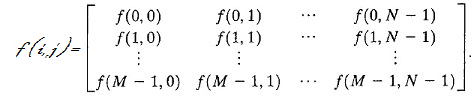
\includegraphics[width=0.7	\textwidth]{./Figures/cap3/id2.png}
%	\caption{Representación de una imagen digital.}
%	\label{fig:green}
%\end{figure}
\nomenclature[1]{$f$}{Función que representa una imagen digital.}%
\nomenclature[2]{$f(i,j)$}{Intensidad del píxel de la fila $i$ y columna $j$ de la imagen digital.}%
\nomenclature[2]{$(i,j)$}{Píxel en la la fila $i$ y columna $j$  de la imagen.}%


%\subsection{Canal Verde}
%Debido a que la mayoría de los algoritmos de visión por computadora se llevan a cabo utilizando imágenes monocromáticas (binarias y en escalas de grises) \cite{gonzalezdigital,gonzales2002digital}, además de los parámetros a color $RGB$ no son necesarios en nuestra clasificación, se decidió convertir la imagen $RGB$ en una imagen en escala de grises, como se muestra en la FIGURA \ref{fig:green}.

%La conversión del espacio de color también se puede realizar en cada uno de los planos de una imagen a color $RGB$, en este caso se hace con la conversión con el canal Verde.

  %\begin{figure}[H]
%	\centering
%		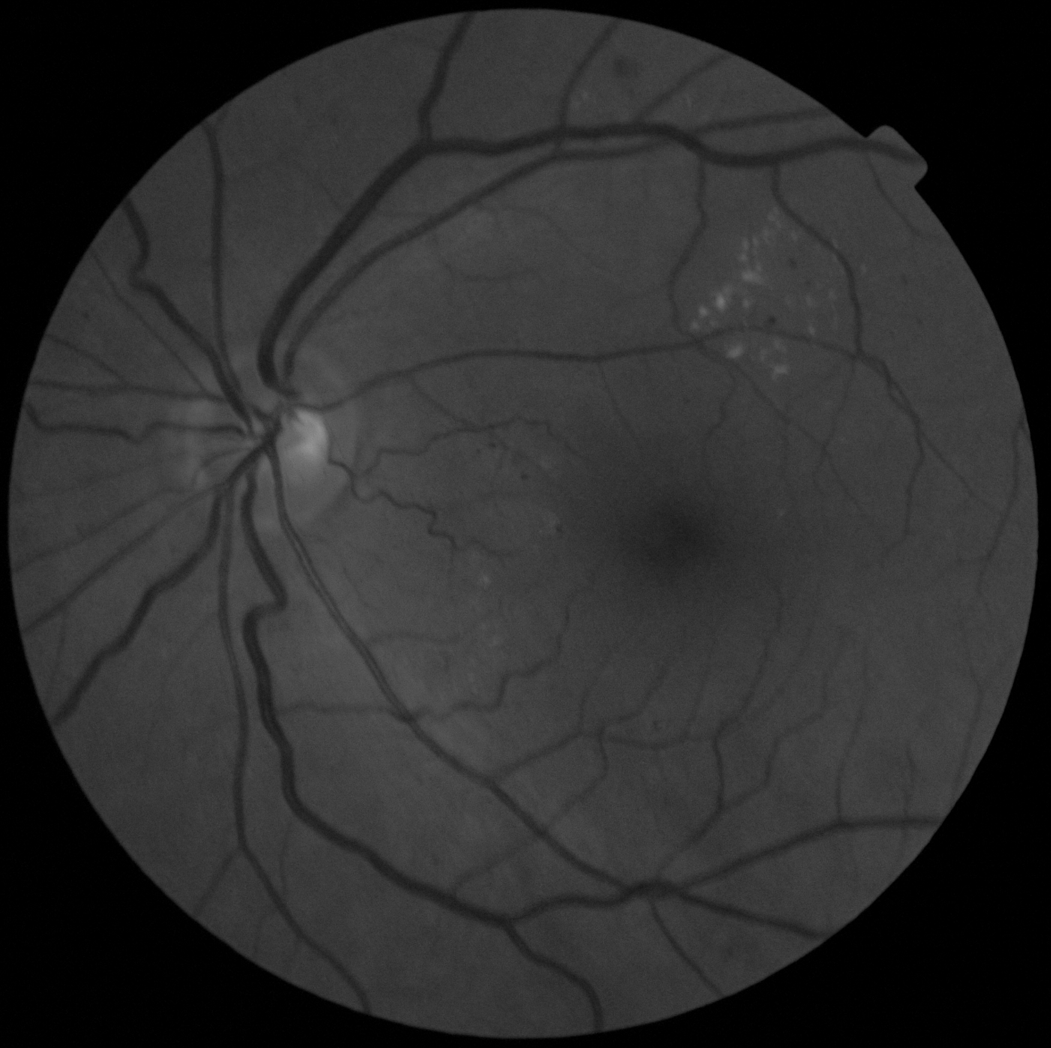
\includegraphics[width=0.4	\textwidth]{./Figures/greenChannel.png}
%	\caption{Canal Verde}
%	\label{fig:green}
%\end{figure}


\section{Vecindad}
Un pixel $r$ de coordenadas $(i,j)$ tiene 4 vecinos horizontales y verticales con coordenadas dadas por:
\begin{equation}
\label{eq:vec}
(i,j+1),(i,j-1),(i+1,j),(i-1,j)
\end{equation}

Los cuales se denominan los 4-vecinos de $r$, y se representan $N_{4}(r)$.
Los 4-vecinos horizontales y verticales, junto a los 4-vecinos en diagonal del
pixel $r$ con coordenadas dadas por:
\begin{equation}
\label{eq:vec1}
(i+1,j+1),(i+1,j-1),(i-1,j+1),(i-1,j-1)
\end{equation}

se denominan los 8-vecinos de $r$ y se representan $N_{8}(r)$.
\nomenclature[3]{$N_{4}(r)$}{Función que representa los 4-vecinos de un píxel $r$.}%
\nomenclature[4]{$N_{8}(r)$}{Función que representa los 8-vecinos de un píxel $r$.}%
  \section{Conectividad}
El concepto de conectividad entre píxeles se emplea para establecer los límites de los objetos. Para saber si 2 píxeles están conectados, debe determinarse si son vecinos entre sí, y su nivel de gris tienen similitud (como ser iguales).
Sea $U$ el conjunto de valores de nivel de gris para establecer conectividad. Por ejemplo en una imagen binaria, $U = {1}$ para la conectividad entre píxeles con valor $1$. En escala de grises se considera un rango de valores de intensidad, por ejemplo $U = {16,17,18,19,20}$ para rangos de $16$ a $20$. Se consideran dos tipos de conectividad:

\begin{enumerate}
 \item 4-conectividad. Dos píxeles $r$ y $q$ con valores dentro de $U$ están 4-conectados si $q$ pertenece a $N_{4}(r)$.
 \item 8-conectividad. Dos píxeles $r$ y $q$ con valores dentro de $U$ están 8-conectados si $q$ pertenece a $N_{8}(r)$.

\end{enumerate}
Un pixel $r$ es adyacente de un píxel $q$ si están conectados. Un camino entre píxeles $r_{1}$ y $r_{n}$ es una secuencia de píxeles $r_{1}, r_{2},..., r_{n-1}, r_{n}$ tal que $r_{k}$  es adyacente a $r_{k+1}$, para $1\leq k < n$. Un camino puede ser 4-conectado o 8-conectado, dependiendo de la definición de adyacencia.
  \section{Componentes conectados}

  Si $r$ y $q$ son píxeles de un subconjunto $S$ especificado de la imagen, se dirá que $r$ está conectado con $q$ dentro de $S$ si existe un camino desde $r$ hasta $q$ que consista totalmente de píxeles de $S$. Para cualquier píxel $r$ dentro de $S$, el conjunto de píxeles de $S$ conectados a $r$ se denomina componentes conectados de $S$.
El etiquetado de componentes conectados consiste en asignar etiquetas distintas a componentes conectados distintos. En la FIGURA \ref{fig:v1a} se puede ver una imagen con componentes conectados y en la FIGURA \ref{fig:v2a} el etiquetado de componentes conectados de esta imagen con 8-vecindad. 
%En la siguiente sección se estará hablando del espacio de color utilizado.
%\cite{hernandezalternativa}.
  
  \begin{figure}[H]
	\centering
	 \subfigure[\label{fig:v1a}]{	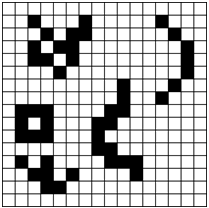
\includegraphics[width=0.15 \textwidth ]{./Figures/ejemploVecindad1.png}}
	\subfigure[\label{fig:v2a}]{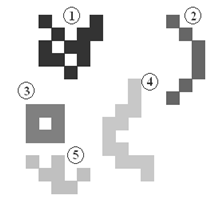
\includegraphics[width=0.15\textwidth  ]{./Figures/ejemploVecindad2.png}}
		\caption{(a) Imagen con componentes conectados, (b) Etiquetado de componentes conectados.}
	\label{fig:ejemploVecindad}
\end{figure}

  
 %   \begin{figure}[H]
%	\centering
%		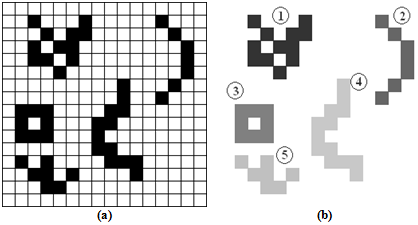
\includegraphics[width=0.5	\textwidth]{./Figures/ejemploVecindad.PNG}
%	\caption{Ejemplo de Etiquetado de componentes conectadas de Vecindad.}
%	\label{fig:ejemploVecindad}
%\end{figure}
 
%\subsection{Canal intensidad ??}
%\section{Espacio de Colores}
%Los espacios de color proporcionan un método para especificar, ordenar y manipular colores. Estas representaciones se corresponden con n-dimensional ordenaciones de las sensaciones de color (vectores de n componentes). Los colores se representan mediante puntos en estos espacios. Existen numerosos espacios de color en la actualidad. La gran mayoría de ellos se han  desarrollado para aplicaciones específicas, aunque todos parten de un mismo concepto: la teoría  tricromática de colores primarios rojo, verde y azul \cite{ortiz2002procesamiento}.

%El color es una característica importante para la clasificación y descripción de objetos en la visión por computadora. Existen diferentes modelos de color los cuales se describen a continuación:
\section{Espacio de color RGB}


%El primero de los modelos de color a comentar y más comúnmente empleado es el RGB, por sus siglas en inglés (Red, Green, Blue), basado directamente en el modelo triestímulos y síntesis aditiva. Es un modelo de color dependiente de dispositivo. 

En el espacio $RGB$ (Red, Green Blue) el color aparece especificado mediante cantidades positivas de rojo, verde y azul, formando en el espacio 3D el cubo que se presenta en la FIGURA \ref{fig:refEspRGB}. El rango de cada coordenada o componente cromática $RGB$ suele estar en [0,1]. %aunque en multimedia y procesamiento de imágenes está más extendida la especificación en cantidades discretas presentes en el intervalo [0,255]. 
Todas las coordenadas que se extienden en la línea que parte del punto ‘negro’ al ‘blanco’ corresponden a la escala de los grises \cite{ortiz2002procesamiento}. 

 \begin{figure}[H]
	\centering
		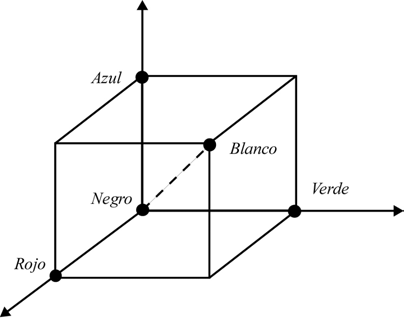
\includegraphics[width=0.4	\textwidth]{./Figures/cap3/RepreEspacialRGB.png}
	\caption{Representación espacial del modelo de color RGB.}
	\label{fig:refEspRGB}
\end{figure}

La mezcla de colores, definidas por sus longitudes de onda luz, normalmente rojo, verde y azul se realiza utilizando la mezcla aditiva de colores,
también referido como el modelo $RGB$ o el espacio de color $RGB$.
\nomenclature[5]{$M$}{Número de filas de la imagen.}%
\nomenclature[6]{$N$}{Número de columas de la imagen.}%
Una imagen a color RGB es representada por una matriz tridimensional $M \times N \times 3$ donde $M$ representa el número de filas, $N$ el número de columnas y 3 representa la cantidad de canales, ver FIGURA. \ref{fig:mezclaAditiva} %\cite{andrews1972image}.
 \begin{figure}[H]
	\centering

		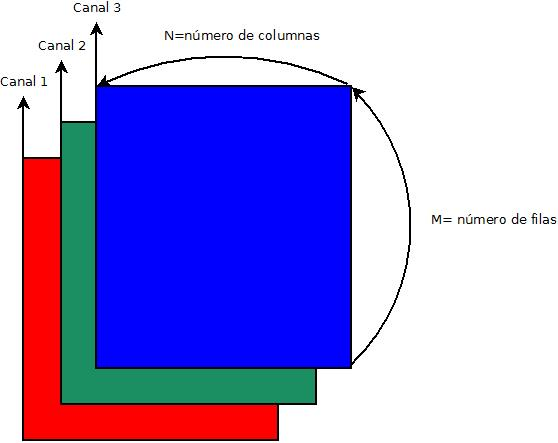
\includegraphics[width=0.65	\textwidth]{./Figures/cap3/mnP.jpeg}
	\caption{Representación de una imagen en RGB.}

	\label{fig:mezclaAditiva}
\end{figure}
\nomenclature[7]{$I$}{Intensidad media de los 3 canales de una imagen RGB.}%

La intensidad $I$ es una magnitud fácilmente deducible de los valores $RGB$. Es el promedio de los 3 canales: rojo, verde y azul como se puede observar en la siguiente ecuación:

\begin{equation}
\centering
\label{eq:intensidad}
I=\frac{I_{Red}+I_{Green}+I_{Blue}}{3}
\end{equation}

\nomenclature[8]{$I_{Red}$}{Canal rojo de la imagen RGB.}%
\nomenclature[9]{$I_{Green}$}{Canal verde de una imagen RGB.}%
\nomenclature[10]{$I_{Blue}$}{Canal azul de una imagen RGB.}%
donde $I_{Red}$, $I_{Green}$, $I_{Blue}$ indican las intensidades de cada canal respectivamente.
\section{Pre-procesamiento de imágenes}

Son pasos previos que se aplican sobre las imágenes para corregir niveles bajos de iluminación, la reflexión sobre los objetos y el ruido aleatorio, que hacen que las imágenes no presenten siempre una buena calidad. Esto se realiza mediante técnicas de reducción del ruido y técnicas de realce de contraste \cite{alvarez2006preprocesamiento}.
El objetivo del pre procesamiento es mejorar la calidad de las imágenes para su posterior utilización  o interpretación  \cite{de2001vision}. A continuación se describen  los métodos de pre-procesamiento utilizados en este trabajo.

\subsection{Métodos en el dominio espacial}
Los métodos en el dominio espacial operan directamente sobre los píxeles. Las funciones en el dominio espacial se expresan como:
\nomenclature[11]{$T_e$}{Función de operador espacial definido alrededor del píxel $(i,j)$.}%

\nomenclature[12]{$g$}{Función que representa una imagen de salida.}%

\begin{equation}
\centering
\label{eq:metDomEsp}
g(i,j)=T_e(f(i,j))
\end{equation}

donde $f$ es la imagen de entrada, $g$ es la imagen procesada y $T_e$ es un operador que actúa sobre $f$, definido en algún entorno de $(i,j)$.
La aproximación principal para definir un entorno alrededor de $f(i,j)$ es emplear un área de subimagen cuadrada (o máscaras espaciales) en $(i,j)$, como se muestra en la FIGURA \ref{fig:metDomEsp}. 

\begin{figure}[H]
	\centering
		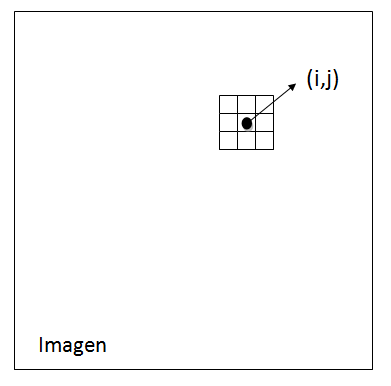
\includegraphics[width=0.5	\textwidth]{./Figures/cap3/m.PNG}
	\caption{Vecindario $3\times3$ de un punto $(i,j)$ de una imagen.}
	\label{fig:metDomEsp}
\end{figure}

\subsection{Filtros}
Los filtros o máscaras espaciales se aplican a una imagen digital para mejorarla o resaltar cierta información.
La FIGURA \ref{fig:mascara3x3} muestra una máscara $3\times3$ general, donde $w_{1}$, $w_{2}$, ..., $w_{9}$ indican los pesos asociados a las coordenadas de las casillas.


\begin{figure}[H]
	\centering

		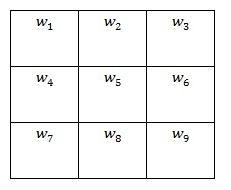
\includegraphics[width=0.4	\textwidth]{./Figures/cap3/mascara.png}
	\caption{Máscara $3\times3$ con coeficientes (pesos) arbitrarios.}

	\label{fig:mascara3x3}
\end{figure}


\subsection{Filtrado}
Son operaciones que se aplican a los píxeles de una imagen para optimizarla, enfatizar cierta información o conseguir un efecto especial en la imagen.  
A partir de una imagen origen, se obtiene una imagen final cuyo resultado sea más adecuado para una aplicación específica.
La aplicación de filtros busca:
\begin{itemize}
\item Suavizar la imagen: minimizar las variaciones de intensidad entre píxeles vecinos.
\item Eliminar ruido: elimina los píxeles con nivel de intensidad muy distinto al de sus vecinos y cuyo origen puede estar tanto en el proceso de adquisición de la imagen como en el de transmisión.
\item Realzar bordes: destacar los bordes que se localizan en una imagen.
\item Detectar bordes: detectar los píxeles donde se produce un cambio brusco en la función intensidad.
\end{itemize}
 
\subsubsection{Filtrado lineal}
Con independencia del tipo de filtro lineal empleado, el enfoque básico
consiste en sumar productos entre los coeficientes de la máscara y las intensidades
de los píxeles bajo la máscara en un punto determinado de la imagen.
Una máscara lineal se define como:

\begin{equation}
\centering
\label{eq:filtradoLineal}
g(i,j)=\sum_{c_1=0}^{m_w} \sum_{c_2=0}^{n_w} f(i+c1-\frac{n_w}{2},j+c2-\frac{n_w}{2})*w(c1,c2)
\end{equation}
donde  $m_w$ es el número de filas de la máscara, $n_w$ es el número de columnas de la máscara y $w$ es la máscara a aplicar sobre una imagen $f$, en la posición $(i,j)$.
%\nomenclature[13]{$z_i$}{Intensidad de un píxel bajo la máscara en la posición $(i,j)$.}
%\nomenclature[14]{$S_m$}{Sumatoria de los productos de los coeficientes de la máscara por las intensidades bajo la máscara.}%
	\nomenclature[15]{$w(k,l)$}{Coeficiente arbitrario de la máscara en la posición $(k,l)$. }%

    Con respecto a la FIGURA \ref{fig:metDomEsp}, si el centro de la máscara de $ 3\times 3$ se encuentra en un
punto $(i,j)$ de la imagen, el nivel de gris del píxel situado en $(i,j)$ se remplaza
por el valor acomulado en  (\ref{eq:filtradoLineal}). Luego se mueve la máscara hasta el emplazamiento del siguiente píxel de la imagen y se repite el proceso. Se continúa así hasta que se
han cubierto todos los píxeles de la imagen.


\subsubsection{Filtrado no lineal}
Los filtros espaciales no lineales operan en los valores de los píxeles en el entorno en consideración y no utilizan los coeficientes de la forma descrita en la ecuación (\ref{eq:filtradoLineal}).


\subsection{Filtro de la mediana}
El filtro de la mediana, sustituye al valor de un píxel por la mediana de los niveles de gris en la vecindad de ese píxel. La mediana es el valor para el cual el 50\% de todos los píxeles en el histograma son mayores y 50\% son menores, al contrario de la media ésta no es influenciada por los valores máximos o mínimos \cite{mehl1997fundamentos,gupta2011algorithm}.

El valor original del píxel está incluido en el cálculo de la mediana. Los filtros de la mediana son muy populares debido a que, para ciertos tipos de ruido aleatorio que proporcionan excelentes capacidades de reducción de ruido. El funcionamiento del filtro de la mediana se puede ver en la FIGURA \ref{fig:FiltroDeLaMediana}. En la FIGURA \ref{fig:medFilt1} se puede ver una imagen con ruido que pueden ver como pequeños puntos blancos y en la FIGURA \ref{fig:medFilt2} se ve el resultado de aplicarle a dicha imagen el filtro de la mediana y como se puede ver remueve el ruido de la imagen.



\begin{figure}[H]
	\centering
		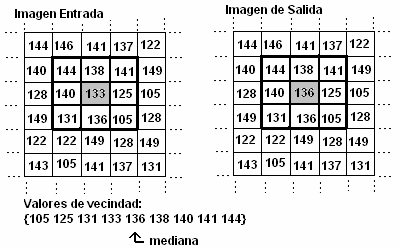
\includegraphics[width=0.6	\textwidth]{./Figures/cap3/FiltrodelaMediana.png}
	\caption{Operación del filtro de la mediana.}
	\label{fig:FiltroDeLaMediana}
\end{figure}

%En la FIGURA \ref{fig:medFilt} se muestra una imagen en la cual se elimina el ruido aplicando el filtro de la mediana.


  \begin{figure}[H]
	\centering
	 \subfigure[\label{fig:medFilt1}]{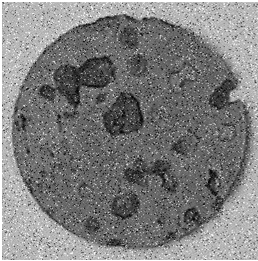
\includegraphics[width=0.3	\textwidth]{./Figures/cap3/OriginalMedian.png}}
	\subfigure[\label{fig:medFilt2}]
	{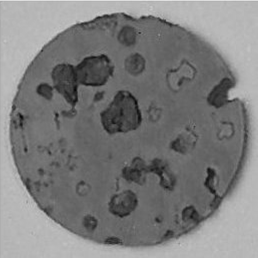
\includegraphics[width=0.3	\textwidth]
	{./Figures/cap3/medianFilteredImage.png}
	}
	\caption{Filtro de la mediana (a) Imagen de entrada y (b) Imagen filtrada.}
	\label{fig:medFilt}
\end{figure}




\subsection{Ajuste de los valores de intensidad}

El ajuste de los valores de intensidad es el ajuste  de los valores de intensidad de una imagen (combinación del brillo y el contraste) con el objetivo de compensar las variaciones de los dispositivos de salida. Básicamente, este proceso ajusta las de intensidades en imágenes en escala de grises y consiste en delimitar un intervalo de intensidades. Las intensidades que se encuentran dentro del intervalo delimitado pueden ser mapeadas a nuevos valores, de acuerdo a 
una curva establecida por el usuario.
%Dicha curva está definida por cinco parámetros, el factor gamma $\gamma$, $Vbajo_{salida}$, $Valto_{salida}$, $Vbajo_{entrada}$ y $Valto_{entrada}$, donde $Valto_{salida}$ y $Vbajo_{salida}$ delimitan el intervalo de valores de intensidad que se modificaran, mientras que el factor $\gamma$, $Vbajo_{entrada}$ y $Valto_{entrada}$ indican la forma de la curva \cite{gonzalezdigital}.
 En la FIGURA \ref{fig:ajuste1} se ve la imagen de una niña con poca atenuación y colores no intensificados y en la FIGURA \ref{fig:ajuste2} se ve la misma imagen con ajuste de intensidad, %para $\gamma=1$
  como se puede ver la imagen contiene colores más intensificados y mejor atenuación.% En la FIGURA \ref{fig:curvaAjustInt1} se ve la curva generada para $\gamma<1$, en la FIGURA \ref{fig:curvaAjustInt2} se ve la curva generada para $\gamma=1$ y en la FIGURA \ref{fig:curvaAjustInt3} se ve la curva generada para $\gamma>1$.
 \begin{figure}[H]
	\centering
	 \subfigure[\label{fig:ajuste1}]{	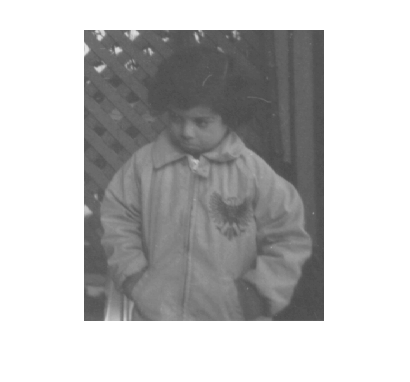
\includegraphics[width=0.3	\textwidth]{./Figures/cap3/Adjust01.png}}
	\subfigure[\label{fig:ajuste2}]{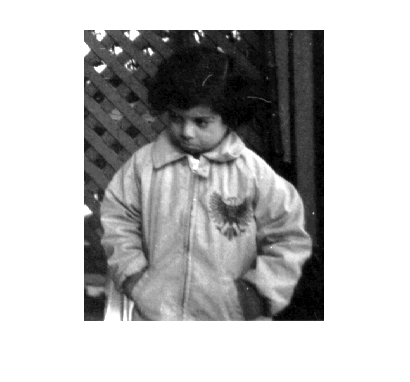
\includegraphics[width=0.3	\textwidth]{./Figures/cap3/Adjust02.png}}
	\caption{Ajuste de intensidad (a) Imagen de entrada y (b) Imagen ajustada.}
	\label{fig:ajuste}
\end{figure}

%\begin{figure}[H]
%	\centering
%	 \subfigure[\label{fig:curvaAjustInt1}]{	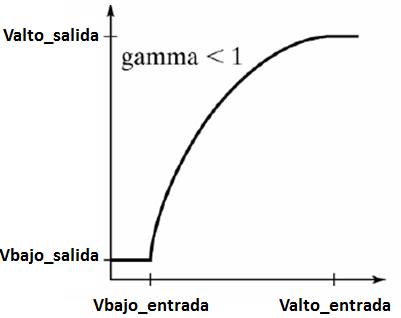
\includegraphics[width=0.3	\textwidth]{./Figures/cap3/curvasAjusteContraste1.png}}
%	\subfigure[\label{fig:curvaAjustInt2}]{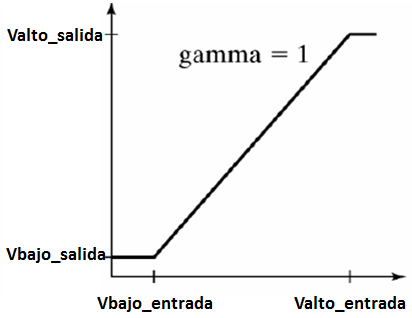
\includegraphics[width=0.3	\textwidth]{./Figures/cap3/curvasAjusteContraste2.png}}
%		\subfigure[\label{fig:curvaAjustInt3}]{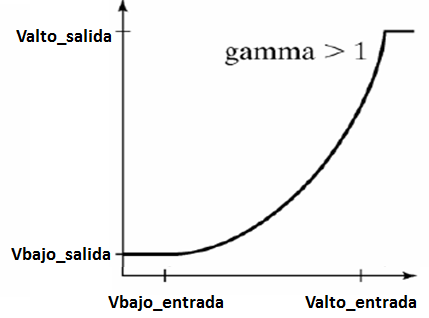
\includegraphics[width=0.3	\textwidth]{./Figures/cap3/curvasAjusteContraste3.png}}
%	\caption{(a) Curva generada para $\gamma<1$, (b) Curva generada para $\gamma=1$ y (c) Curva generada para $\gamma>1$  }
%	\label{fig:CURVAajuste}
%\end{figure}


%\begin{figure}[H]
%	\centering
%		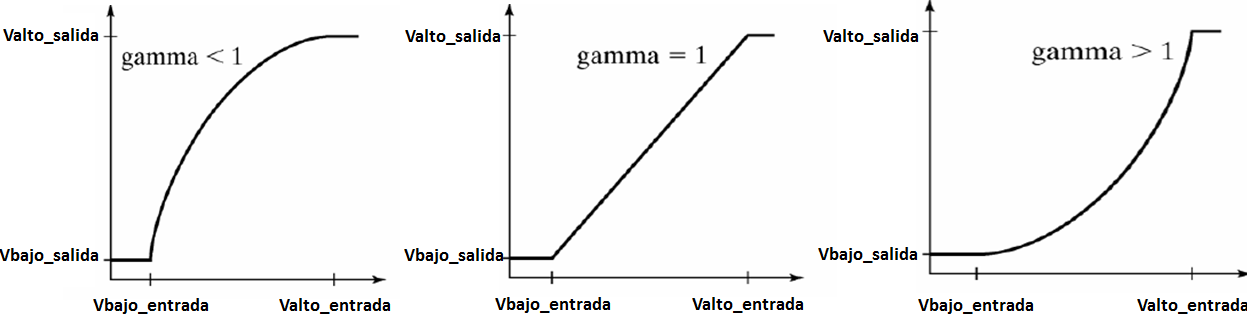
\includegraphics[width=0.8	\textwidth]{./Figures/cap3/curvasAjusteContraste.png}
%	\caption{Curvas generadas en base al factor $\gamma$}
%	\label{fig:curvaAjustInt}
%\end{figure}


\subsection{Histograma de una imagen }


%El   histograma   de   una   imagen   es   ampliamente   utilizado   como   herramienta   tanto cualitativa como cuantitativa.%
El   histograma   de   una   imagen corresponde a un gráfico de la distribución de valores  de intensidad de los píxeles  de  la  imagen (niveles de gris) o de una porción de la misma. 
\nomenclature[16]{$H$}{Función de histograma de una imagen.}%
\nomenclature[17]{$L$}{Máximo valor de intensidad.}%
\nomenclature[18]{$n_{k}$}{Número de ocurrencia de la intensidad $k$ en la imagen.}%

Para una imagen $f$, dada de dimensión $ M\times N$ píxeles, donde $f(i,j)$ representa la intensidad de un píxel dentro de la imagen y siendo $(i,j)$ las coordenadas espaciales del píxel dentro de la imagen, el histograma $H$ (ver FIGURA
\ref{fig:histogram}) asociado a la imagen que describe la frecuencia de los valores de intensidades que aparecen en la misma, donde $k=0,1,....,L-1$ se define como:
\begin{equation}
\label{eq:histFormalEquation}
H(k)=n_{k}
\end{equation}

donde $L-1$ representa el nivel máximo de gris en una imagen y $n_{k}$ representa el número de ocurrencia de la intensidad $k$ en
la imagen.

%Podemos  denotar como $H(i)$, el número de píxeles que dentro de la región de interés tiene el valor de intensidad $i$, donde $i = 0, 1, 2, ...., L -1$, donde $L$ representa el nivel máximo de gris en una imagen. Los valores $H(i$), corresponderán entonces a los valores del histograma. El gráfico del histograma  es  bidimensional  y  en  él  se  gráfica  $H$  en  función  de  $i$.  Tal  gráfico,  puede proporcionar una importante información acerca del brillo y contraste de una imagen así como de su rango dinámico. En la FIGURA \ref{fig:histogram} se muestra un histograma típico \cite{medina1997bases}.

\begin{figure}[H]
	\centering
		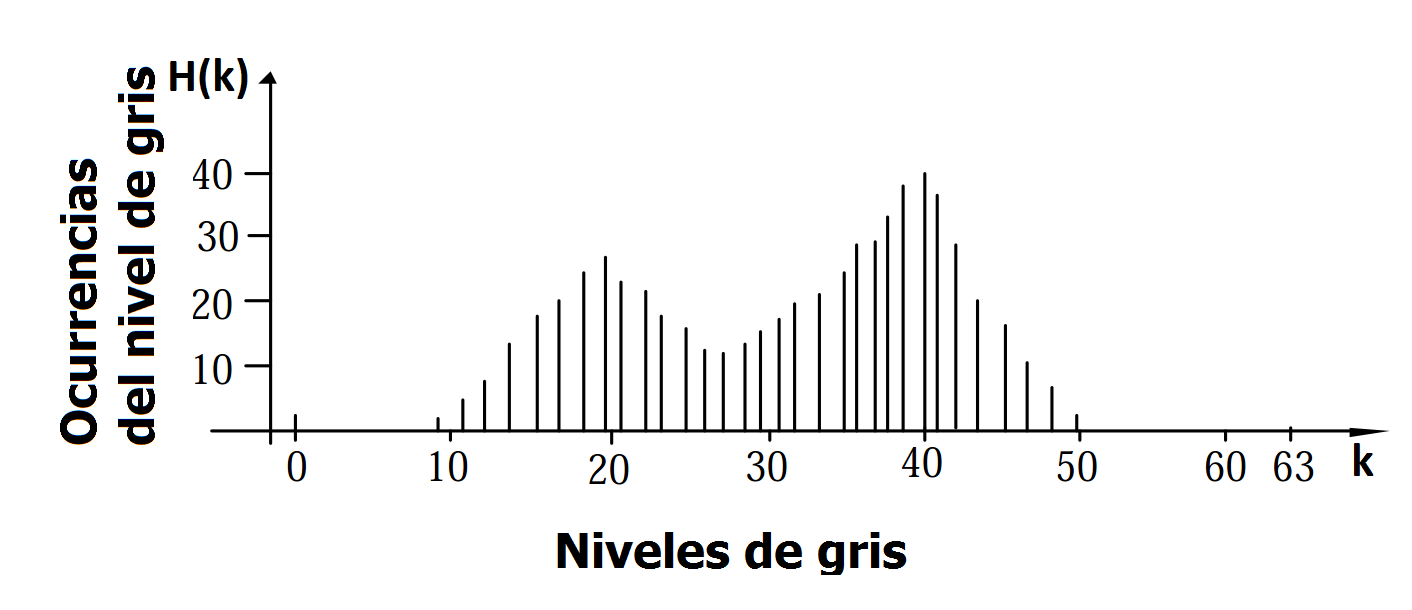
\includegraphics[width=0.6	\textwidth]{./Figures/cap3/Histograma.PNG}
	\caption{Histograma para los niveles de intensidad de una imagen con L=64.}
	\label{fig:histogram}
\end{figure}

\subsection{Ecualización del histograma (HE)}
%Considere una imagen discreta  en escala de grises ${ f }$ y dejar que $n_{i}$ sea el número de ocurrencias de nivel de gris $i$ . La probabilidad de una ocurrencia de un píxel de nivel $i$ en la imagen es:

%\begin{equation}
%\label{eq:he}
%p_x(i) = p(x=i) = \frac{n_i}{n},\quad 0 \le i < L
%\end{equation}

%L es el número total de niveles de gris en la imagen (normalmente 256), n es el número total de píxeles de la imagen, y $P_X(i)$ siendo el histograma de la imagen para el valor de píxel i, normalizado a [0,1].

%También debemos definir la función de distribución acumulada correspondiente a $p_x$ como:


%\begin{equation}
%\label{eq:funDistAcum}
%cdf_x(i) = \sum_{j=0}^i p_x(j)
%\end{equation}

%que también es acumulada histograma normalizado de la imagen.
%Se crea una transformación de tal forma que $y=T(x)$ para producir una nueva imagen ${y}$, con un histograma plano. Tal imagen tendría un CDF linealizado a través de la gama de valores, es decir,

%\begin{equation}
%\label{eq:constanteK}
%cdf_y(i) = iK
%\end{equation}


%para alguna constante K. Las propiedades del CDF nos permiten realizar una transformación que se define como:

%\begin{equation}
%\label{eq:funTransCDF}
%cdf_y(y^\prime) = cdf_y(T(k)) = cdf_x(k)
%\end{equation}

%donde k está en el rango [0, L). T aplica los niveles en el rango [0,1], ya que utilizamos un histograma normalizado de {x}. Con el fin de mapear los valores de nuevo en su rango original, la siguiente transformación sencilla necesita ser aplicada en el resultado:

%\begin{equation}
%\label{eq:tranSenc}
%y^\prime = y \cdot(\max\{x\} - \min\{x\}) + \min\{x\}
%\end{equation}
\nomenclature[19]{$p(k)$}{Función de densidad de probabilidad de la intensidad $k$ asociada a $H$.}%

En la ecualización del histograma (HE del inglés $Histogram Equalization$) se identifica la función de densidad de probabilidad $p(k)$ asociada a $H$ dada por:
\begin{equation}
\label{eq:funDenProbAsociada}
p(k)=\frac{H(k)}{M\times N}
\end{equation}
donde $p(k)$ indica la probabilidad de aparición de la k-ésima intensidad. Mientras que su función de densidad acumulada
$c(k)$ esta dada por:
\nomenclature[20]{$c(k)$}{Función de densidad acumulada de probabilidad de la intensidad $k$ asociada a $H$.}%
\begin{equation}
\label{eq:FunDenAcumulada}
c(k)=\sum_{i=F_{0}}^{k}p(i)
\end{equation}
\nomenclature[21]{$F_{0}$}{Menor intensidad en el rango de cálculo de la densidad acumulada.}
\nomenclature[22]{$F_{max}$}{Mayor intensidad en el rango de cálculo de la densidad acumulada.}
\nomenclature[23]{$ac$}{Función de arreglo de acumulación.}%
donde $F_{0}$ es la menor intensidad dentro del rango que se desea calcular la función de densidad acumulada.
La función de transformación $T_{HE}(k)$ asociada a la ecualización de histograma estándar mapea la imagen de entrada al rango dinámico $[F_{0},F_{max}]$, usando $c(k)$. La función está dada por la siguiente ecuación:
\begin{equation}
\label{eq:histo_4}
T_{HE}(k)=F_{0}+(F_{max}-F_{0})\times c(k)
\end{equation}

\nomenclature[24]{$T_{HE}$}{Función de transformación asociada a la ecualización del histograma.}%
para el caso particular de la ecualización del histograma, el rango esta dado por $F_{0}=0$ y $F_{max}=L-1$. Así, la imagen resultante producida por la
ecualización del histograma, $g$, puede ser expresada como:
\begin{equation}
\label{eq:histo_5}
 g(x, y) = T_{HE} (f(x, y)) \text{  }  \forall  f(x, y) \in  f
\end{equation}

Usando sólo información  global no logra buen realce de contraste, debido a 
que las técnicas globales causan efecto de saturación de intensidades \cite{wang2007fast}. Para solucionar este problema existe una ecualización del histograma localizada o también conocida como adaptativa.
 En la FIGURA \ref{fig:he1} se ve la imagen de una rueda con poco contraste y en la FIGURA \ref{fig:he2} se ve la misma imagen ecualizada y en la misma se puede notar una mejora de contraste. 
\begin{figure}[H]
	\centering
	 \subfigure[\label{fig:he1}]{	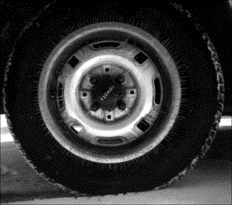
\includegraphics[width=0.3	\textwidth]{./Figures/cap3/tire.png}}
	\subfigure[\label{fig:he2}]{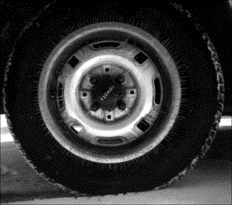
\includegraphics[width=0.3	\textwidth]{./Figures/cap3/tire.png}}
	\caption{Ecualización del histograma (a) Imagen de entrada y (b) Imagen ecualizada.}
	\label{fig:he}
\end{figure}

\subsection{Ecualización del histograma adaptativo}
En AHE (\textit{Adaptive Histogram Equalization}), se optimiza el contraste dentro de regiones rectangulares de la imagen, llamadas
regiones contextuales o ventanas, con dimensiones definidas. La
ecualización del histograma se realiza en cada región contextual de forma independiente.
La ecualización adaptativa  considera una ventana local para cada píxel y calcula el valor de la nueva intensidad basado en el histograma local definido para  cada ventana. Una deficiencia del AHE es que amplifica el ruido, siendo solucionado esto por medio de la ecualización del histograma adaptativo de contraste limitado o CLAHE (\textit{Contrast Limited Adaptive Histogram Equalization}).
%Para ecualizar una imagen de entrada $x$, con niveles de  grises cuantizados, primero se estima el histograma local $\hat h$. Para esto se inicia por evaluar los niveles de grises de  la imagen de entrada usando la función delta Kronecker $\delta(i,j)$, la cual es igual a 1 si i=j y 0 en otros casos. La  convolución espacial con una máscara rectangular$ f\omega $ puede ser usada para encontrar aquellos píxeles en una  ventana alrededor de cada punto. Para una ventana  cuadrada de ancho $\omega $ y con un número de componentes  PARES, el histograma local puede ser escrito como [7]:
%\begin{equation}
%\label{eq:ah1}
%\hat h(m,n,g)=\delta (g,x(n,m))\otimes f_{\omega }(m,n)
%\end{equation}
%\begin{equation}
%\label{eq:ahe2}
%f_{\omega }(m,n)=\begin{cases}
% & \omega ^{-2} | m | \leq \frac{\omega -1}{2} \text{ y } \omega ^{-2} | n | \leq \frac{\omega -1}{2}  \\ 
% &  0  \text{ en otro caso  } 
%\end{cases}
%\end{equation}
%La imagen de salida se calcula usando:
%\begin{equation}
%\label{eq:ahe3}
%y(m,n)=z(m,n,x(m,n))
%\end{equation}
%Donde z es la variación de reescalado espacial y se obtiene a partir de la expresión:
%\begin{equation}
%\label{eq:ahe4}
%z(m,n,g)=\frac{1}{2}\sum_{y=g_{0}}^{y\leq g} \hat h(m,n,\gamma) -\frac{1}{2}\sum_{y=g_{0}}^{y\leqg} \hat h(m,n,\gamma)
%\end{equation}
\subsection{Ecualización del histograma adaptativo de contraste limitado}
CLAHE fue desarrollado originalmente para mejora de imágenes médicas y prevenir la amplificación de ruido que no se podía evitar en el AHE \cite{pizer1987adaptive}.
CLAHE difiere del AHE convencional en que el contraste se limita. El procedimiento de limitar el contraste tiene que ser aplicado a cada vecindario. Subsana el problema limitando la cantidad de píxeles que puede alcanzar determinado nivel de gris \cite{singh2011analysis}. En la FIGURA \ref{fig:clahe1} se ve una imagen poco contrastada, en la FIGURA \ref{fig:ahe1} se ve la ecualización del histograma adaptativo (AHE) de dicha imagen, en la misma se puede notar la amplificación del ruido en ciertas zonas de la imagen. Finalmente en la FIGURA \ref{fig:clahe2}  se ve la imagen poco contrastada tras aplicar CLAHE y se puede ver claramente una mejora con respecto a la reducción del ruido. 
%Esta característica puede también ser aplicado a la ecualización de histograma global, que es raramente utilizado en la práctica. 
%En el caso del CLAHE, 
%CLAHE fue originalmente desarrollado para mejora de imágenes médicas y ha sido muy útil en la mejora de imágenes de contraste bajo. El algoritmo del CLAHE particiona las imágenes en regiones contextuales y aplica la ecualización del histograma a cada uno \cite{singh2011analysis}.
%La expresión de los niveles de gris modificados para el método estándar de CLAHE con distribución uniforme esta dada por:
%\begin{equation}
%\label{eq:clahe}
%g=[g_{max}-g_{min}]*P(f)+g_{min}
%\end{equation}
%Donde $g_{max}$=valor máximo del píxel
%$g_{min}$=valor mínimo del píxel
%$g$=nuevo valor del píxel
%$P(f)=CPD$ (distribucción de probabilidad acumulada)
  \begin{figure}[H]
	\centering
	 \subfigure[\label{fig:clahe1}]{	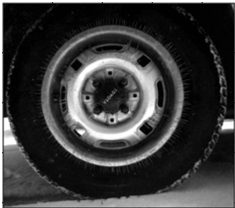
\includegraphics[width=0.3	\textwidth]{./Figures/cap3/clahe1.png}}
	 \subfigure[\label{fig:ahe1}]{	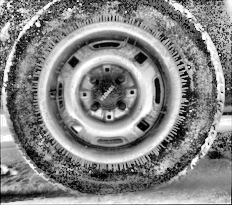
\includegraphics[width=0.3	\textwidth]{./Figures/cap3/ahe1.png}}
	\subfigure[\label{fig:clahe2}]{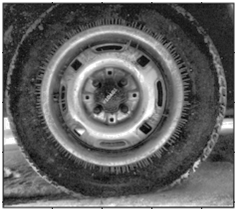
\includegraphics[width=0.3	\textwidth]{./Figures/cap3/clahe2.png}}
	\caption{(a) Imagen de entrada, (b) AHE y (c) CLAHE.}
	\label{fig:clahe}
\end{figure}
    \section{Transformada de Hough}
   La transformada de Hough \cite{ hough1962method} está orientada a la detección de contornos cuya forma básica es conocida y que puede ser representada como una curva paramétrica, tales como líneas, círculos, elipses, cónicas, entre otras. El principio básico de la transformada de Hough es obtener puntos en una imagen. La idea es aplicar una transformación en la imagen de tal manera que todos los puntos que pertenecen a la misma curva sean mapeados a un único punto en un nuevo espacio de parametrización de la curva buscada.
  Es una técnica muy robusta frente al ruido y a la existencia de huecos en la frontera del objeto \cite{platero2009apuntes}. 
  
  En este trabajo se utiliza la transformada de Hough para detectar círculos de radio $r$ en una imagen $f$ de dimensión $M\times N$ donde $M$ es el número de filas y  $N$ es el número de columnas, se va necesitar de un arreglo de acumulación bidimensional $ac$  de dimensión $M \times N$ que será utilizado como contador por ende inicialmente todos sus valores serán $0$. A continuación se describe el pseudocódigo del proceso de detección de círculos utilizado para este trabajo:
  
  Los valores en  $ac$ más altos serán los centros de los círculos detectados.
  
 


%\begin{equation}
%\label{eq:anguloDir}
%\begin{cases}
% & x_{0}=x+ r * \cos \rho   \\  
%& y_{0}=y+ r * \sin\rho 
%\end{cases}
%\end{equation}

  %\begin{equation}
%\label{eq:hough2}
%\begin{cases}
%\text{Si }  \text{ e } 
%\end{cases}
%\end{equation}
  
%  En la FIGURA \ref{fig:mapeoHough} se observa un ejemplo de esta técnica.
 %    \begin{figure}[H]
%	\centering
%	 \subfigure[]{	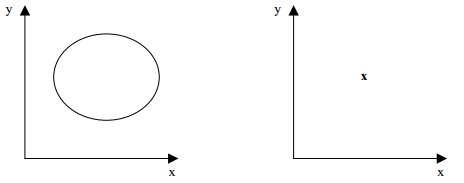
\includegraphics[width=0.7	\textwidth]{./Figures/cap3/mapeoHough.PNG}}

%	\caption{Aplicación de la  TH a una curva cualquiera parametrizada en el espacio $x,y$ mapeada a un único punto.}
%	\label{fig:mapeoHough}
%\end{figure}
 %  Para más sobre el funcionamiento de la transformada de hough para detección de círculos ver  \cite{rojas2008sistema}.
 %  \subsection{Detetcción de círculos}
   
  % Considere el Circulo $\Delta_{1}$ de radio $R$ y centro de coordenadas en $(X_c,Y_c)$ FIGURA \ref{fig:circuloHough}
   
   %     \begin{figure}[H]
%	\centering
%	 \subfigure[]{	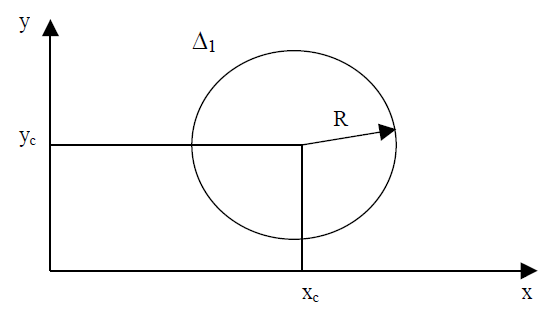
\includegraphics[width=0.7	\textwidth]{./Figures/cap3/houhgCirculo.PNG}}

%	\caption{Circulo $\Delta_{1}$ de radio $R$ y centro de coordenadas en $(X_c,Y_c)$.}
%	\label{fig:circuloHough}
%\end{figure}
%\section{Transformada de Hough: Detetcción de círculos }
    
%La transformada de Hough es una herramienta que permite detectar curvas en una imagen. Es una técnica muy robusta frente al ruido y a la existencia de huecos en la frontera del objeto. \cite{platero2009apuntes}. 

% A continuación se explica la teoría concerniente a la transformada 
%de Hough para detección de círculos. En este trabajo se hace uso de la conocida ecuación paramétrica de un círculo de centro en (i,j)=(a,b) y radio R:

%\begin{equation}
%\label{eq:cia}
%\small	(x-a)^{2}+(y-b)=R^{2}
%\end{equation}

%\subsection{Formulación clásica }
%Independientemente de la formulación de parámetros empleada, la transformada siempre utiliza lo que se conoce como Arreglo de Acumulación, donde se totalizan los “votos” que dan el resultado de los parámetros más apropiados al tipo de forma que se desea detectar \cite{rojas2008sistema}.
%\subsection{Transformada circular de hough}
%El nombre dado a la transformada se deriva del
%tipo específico de FIGURAs a detectar en la imagen: círculos
%\cite{rizon2005object}. Para ello, la descripción de parámetros utilizada
%es,

%\begin{equation}
%\label{eq:descriparams}
%f (x, y, x_{0}, y_{0}, r)= (x -  x_{0})^{2} + (y - %y_{0})^{2} - r^{2}=0
%\end{equation}

%donde la terna $(x0, y0,r)$ conforma el conjunto de parámetros que expande el espacio de Hough a uno tridimensional;
%luego el arreglo de acumulación $H (x0, y0,r)$ será de dimensión 3D. La dirección del gradiente $ \angle G$ puede ser utilizada para reducir los cálculos en el espacio de parámetros de Hough \cite{borovicka2003circle,peng2005detect} y por tanto tener una más eficiente detección, limitando el proceso de votación sólo para los valores de los parámetros que sean más consistentes con la orientación de los bordes de las FIGURAs buscadas en una imagen. Así, en lugar de seleccionar
%votos para todas las rectas que pasan por un punto determinado, se puede escoger votar solamente por aquellas cuya orientación $\varphi$ esté dentro de cierto rango $\o - a \leqslant \varphi \leqslant \o +a$, donde $\o$ es la dirección del gradiente.

%Téngase en cuenta que la dirección del gradiente
%siempre es perpendicular a la dirección tangente de
%una curva dada por $f (x, y) = 0$, como se muestra en %la
%FIGURA\ref{fig:dirGrad}.

%\begin{figure}[H]
%	\centering
%		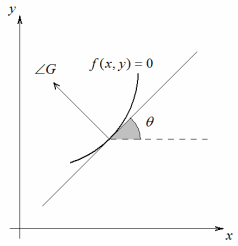
\includegraphics[width=0.4	\textwidth]{./Figures/cap3/direccionGradiente.png}
%	\caption{Dirección del gradiente.}
%	\label{fig:dirGrad}
%\end{figure}

%\begin{equation}
%\label{eq:angulodeDir}
%\tan \Theta = \frac{dy}{dx}=- \frac{f_{x}'(i,j)}{f_{y}'(i,j)}\equiv =g(i,j)
%\end{equation}

%siendo que $\o = \angle G $ y $\theta =\o \pm  \pi/2$

%En forma general, para cualquier tipo de función
%de parámetros resulta:

%\begin{equation}
%\label{eq:funcDeParams}
%\begin{cases}
 %& f(x,y,\alpha_{1},\alpha_{2},...,\alpha_{n} )=0 \\ 
 %&  g(x,y,\alpha_{1},\alpha_{2},...,\alpha_{n} )=-\cot \o 
%\end{cases}
%\end{equation}

%Cualquier punto $(i,j)$ en la imagen de origen,
%corresponde con una superficie en forma de cono en el
%espacio tridimensional, tal como se observa en la FIGURA \ref{fig:espacio3dtranscirc}.

%\begin{figure}[H]
%	\centering
%		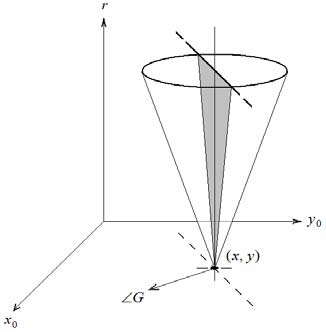
\includegraphics[width=0.6	\textwidth]{./Figures/cap3/Espacio3DTransCircular.png}
%	\caption{Espacio 3D de la transformada circular.}
%	\label{fig:espacio3dtranscirc}
%\end{figure}

%Sobre la base de esta FIGURA y teniendo en cuenta
%la dirección gradiente en los cálculos, según la
%ecuación \ref{eq:funcDeParams}, se tiene:

%\begin{equation}
%\label{eq:dirGradCalc}
%\begin{cases}
 %& (x-x_{0})^{2}+(y-y_{0})^{2}-r^{2}=0 \\ 
 %& (x-x_{0})/(y-y_{0})=\cot \o  
%\end{cases} \rightarrow \begin{cases}
 %& x_{0}=x\pm r*\cos \o   \\ 
 %& y_{0}=y\pm r*\sin \o 
%\end{cases}
%\end{equation}


%\begin{equation}
%\label{eq:anguloDire}
%\o = \angle G=\tan^{-1}(\frac{y_0-y}{x_{0}-x})
%\end{equation}


%Ahora el algoritmo de detección de círculos será: 

%\begin{enumerate}[I]
 %   \item  Iniciar  el  arreglo  de  acumulación  bidimensional  
%del espacio de parámetros de Hough, cuya cantidad 
%de elementos va en función de la resolución de la 
%imagen de origen. 
    
 %  \item Para  cualquier  píxel  que  satisfaga  (  valor  de  referencia del campo gradiente, ajustable experimentalmente), incrementar en uno todos los elementos del 
%arreglo  de  acumulación,  que  cumplan  con  las  dos 
%ecuaciones simultáneas, 

%Para todo r tal que:


    
 %   \item  Cualquier elemento $H(x_{0},y_{0},r)>T_{h}$ (umbral
%de detección, también asignado experimentalmente)
%representará un círculo de radio r y centro en
%$(x_{0}, y_{0})$ contenido en la imagen de origen.
%\end{enumerate}
 

\section{Morfología matemática}
La descripción básica de la Morfología Matemática descansa en la ‘teoría de conjuntos’ cuyos primeros trabajos se deben a Minkowski \cite{minkowski1989allgemeine}  y Hadwiger \cite{der1957vorlesungen,hadwiger1959normale}. 
%La continuación de estos trabajos de investigación, bajo la impulsión y reformulación de Matheron y Serra, se darían posteriormente a conocer bajo la denominación de Morfología Matemática, como una técnica no lineal de tratamiento de señales. La mayor parte de esta teoría ha sido desarrollada en el Centre de Morphologie Mathématique (CMM) de l’Ecole des Mines de Paris. 



La  morfología  matemática  procesa  imágenes con ayuda de una forma especial escogida previamente, el cual generalmente es una matriz más pequeña que la imagen y recibe el nombre de elemento estructurante \cite{sonka2008image,cui2008edge}.
\subsection{Elemento estructurante}
Un elemento estructurante (EE) es un conjunto usado para examinar la imagen. %bajo estudio (FIGURA 3.7). 
El EE se utiliza para investigar la morfología de los objetos presentes en la imagen. 
Cada elemento estructurante requiere la definición de un punto  de origen (o de referencia) para su aplicación como operador morfológico. Esto permite que el elemento estructurante se pueda relacionar de una forma particular con los píxeles de la imagen \cite{sonka2008image},
%Los operadores morfológicos requieren de la definición de un origen para cada EE. Este origen permite el posicionamiento del EE en un determinado punto o pixel. Este centro se sitúa en cada pixel de la imagen original, aplicando la operación morfológica sobre los puntos situados sobre dicho EE. 
el cual actúa, como un operador sobre una imagen para  producir un resultado. La forma,  tamaño  y  orientación  del  elemento  estructurante,  son escogidos  en  base  a  un  conocimiento  previo tomando en  cuenta  las  estructuras  geométricas relevantes  que  estén  presentes  en  la  imagen  y  el  objetivo  que  se  persiga con la operación morfológica implementada \cite{qiu2005image,shih2010image,sonka2008image,cui2008edge}.
Comúnmente EE de 2 dimensiones son llamados EE planos, para más de 2 dimensiones son llamados EE no planos o EE en escala de grises. De manera formal un elemento estructurante se puede definir como una función B(s,t) con centro en $(c,d)$.

 % En la FIGURA \ref{fig:ee} se muestran los elementos estructurantes típicos, donde los centros  están determinados por un punto.  En la FIGURA \ref{fig:ee1} se muestra un elemento estructurante cuadrado, en la FIGURA \ref{fig:ee2} se muestra un elemento estructurante círculo, en la FIGURA \ref{fig:ee3} se muestra un elemento estructurante rombo y en la FIGURA \ref{fig:ee4} se muestra un elemento estructurante línea.
  
    En la FIGURA \ref{fig:ee} se muestran los elementos estructurantes típicos: cuadrado, círculo, rombo y rectángulo y sus centros están determinados por un punto.  

\begin{figure}[H]
	\centering
		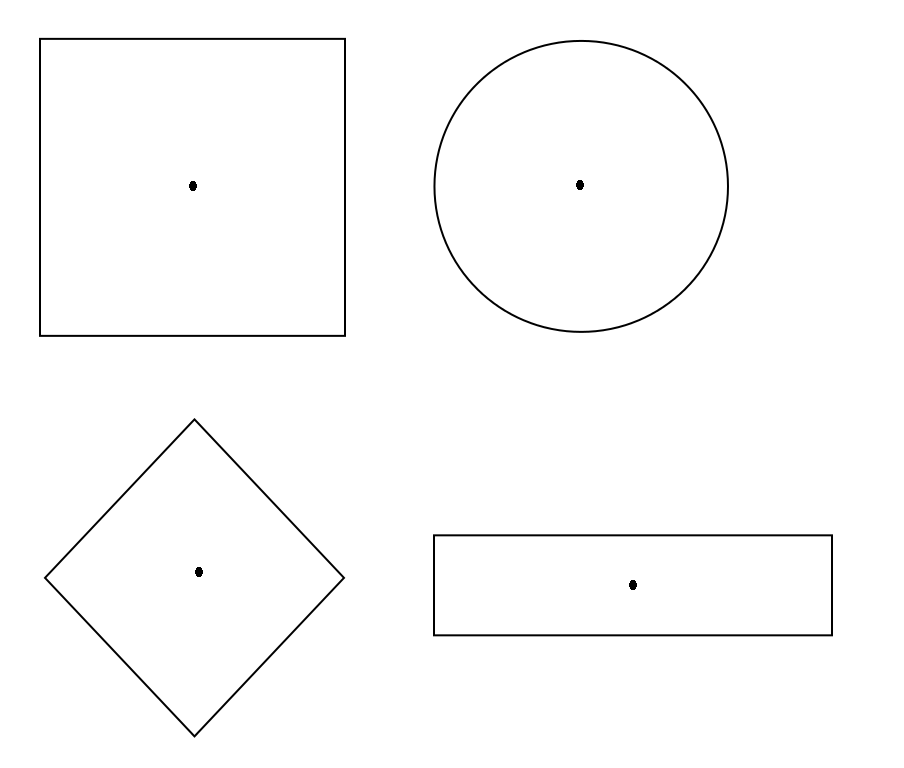
\includegraphics[width=0.6	\textwidth]{./Figures/cap3/ee1.png}
	\caption{Elementos estructurantes típicos: Cuadrado, círculo, rombo y rectángulo.}
	\label{fig:ee}
\end{figure}
   

    \subsection{Dilatación}
    
    
%La dilatación se describe como un crecimiento de píxeles, es decir, se marca con 1 la parte del fondo de la imagen que toque un pixel que forma parte de la región. Esto permite que aumente un pixel alrededor de la circunferencia de cada región y así poder incrementar dimensiones, lo cual ayuda a rellenar hoyos dentro de la región. \cite{bloch1995fuzzy}.

La  dilatación  también  llamada  expansión,  llenado  o  crecimiento,  produce  un  efecto  de engrosamiento en los bordes del objeto. Considerando las imágenes en escala de grises como  superficies $f(i,j)$ y tomando como elemento estructurante $B$, el operador de dilatación se define como:

\begin{equation}
\label{eqa:dilatacionGrises}
f(i,j) \oplus{B} =max \{ f(i+s,j+t)\}  \text{ : } (s,t) \in B 
\end{equation}

%\begin{equation}
%\label{eqa:dilatacionGrises1}
%f(i,j) \oplus{B} =max [ \left ( f(x+s,y+t) | (s,t) \in B ]
%\end{equation}
\nomenclature[25]{$B$}{Elemento estructurante.}%

Es el máximo valor de la imagen $f(i,j)$ en la región coincidente con el elemento estructurante $B$ centrado en $(i,j)$.

%Este algoritmo se utiliza para aumentar el contorno de los   objetos   y   unir   las   líneas   descontinuas   de   estos,   producidas   por   algún   filtrado, 
%\begin{equation}
%\label{eq:dilatacion}
%A\oplus{B} = \bigcup_{b\in{B}}{A_b}
%\end{equation}

%Es decir, dado un elemento estructurante $B$ (formado por unos y ceros), la dilatación de $A$ por $B$ es el  conjunto  de  todos  los  desplazamientos  de  $x$  tales  que  $B$  y  $A$  se  solapen  en  al  menos  un elemento distinto de cero. La FIGURA \ref{fig:dilatacion}, muestra un ejemplo de la dilatación. 
En la FIGURA \ref{fig:dilatacion1} se ve la imagen de un circuito y en la FIGURA \ref{fig:dilatacion2} se ve la misma imagen del circuito en donde se ve el crecimiento de las zonas claras y se redujeron las zonas oscuras tras aplicar la operación de dilatación.




\begin{figure}[H]
	\centering
	 \subfigure[\label{fig:dilatacion1}]{	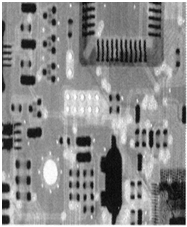
\includegraphics[width=0.3	\textwidth]{./Figures/cap3/gray.png}}
	\subfigure[\label{fig:dilatacion2}]{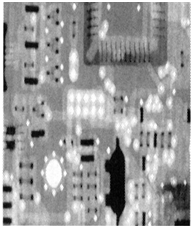
\includegraphics[width=0.3	\textwidth]{./Figures/cap3/dilated.png}}
	\caption{Dilatación en imágenes en escala de grises (a) Imagen de entrada y (b) Imagen dilatada.}
	\label{fig:dilatacion}
\end{figure}

    
    
\subsection{Erosión}
%La erosión de un conjunto $X$ por un elemento estructurante $B$ es denotada por
%$\epsilon _{B}(X)$ y es definida como el lugar geometrico de puntos $x$ tal que $B$ %es incluido en $X$ cuando su origen es puesto en $x$:

 %\begin{equation}
%\label{eq:erosion1}
%\epsilon _{B}(X)= \{ x|B_{x}\subseteq X  \}
%\end{equation}
%La ecuación \ref{eq:erosion1} puede ser expresada en términos de la intersección de un conjunto de traslaciones. Las traslaciones son establecidos por el EE:


La erosión es la función dual de la dilatación, la erosión reduce los contornos de los objetos. Este operador se utiliza típicamente para separar objetos que están unidos por una pequeña parte de sus contornos. Considerando  las  imágenes  en  escala  de  grises  como  superficies   $f(i,j)$ y tomando  como elemento estructurante $B$, se define el operador de erosión como:
\begin{equation}
f(i,j) \ominus{B} =min \{ f(i+s,j+t) \} \text{ : } (s,t) \in B  
\label{eqb:t}
\end{equation} 


Es el mínimo valor de la imagen $f(i,j)$ en la región coincidente con el elemento estructurante $B$ centrado en $(i,j)$.

%matemáticamente la erosión $\ominus$ se define como:

%\begin{equation}
%\label{eq:dilatacion}
%A\ominus{B} = \bigcap_{b\in B}A_{b}
%\end{equation}
 %Es decir, la erosión pone a cero todos los píxeles de la imagen que  no contengan completamente al elemento estructurante en su entorno. La FIGURA \ref{fig:erosion}, muestra un ejemplo de la erosión. 

%Dada una imagen A se erosiona por B cuando para todos los puntos x tales que B, trasladado por x, está contenido en A. 
%Es decir, la erosión pone a cero todos los píxeles de la imagen que  no contengan completamente al elemento estructurante en su entorno.
%Si la dilatación expandía los 
%bordes y contornos de los objetos, 

En la FIGURA \ref{fig:erosion1} se ve la imagen de un circuito y en la FIGURA \ref{fig:erosion2} se ve el crecimiento de las zonas oscuras y la reducción de las zonas claras tras aplicar la operación de erosión.



\begin{figure}[H]
	\centering
	 \subfigure[\label{fig:erosion1}]{	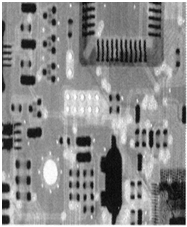
\includegraphics[width=0.3	\textwidth]{./Figures/cap3/gray.png}}
	\subfigure[\label{fig:erosion2}]{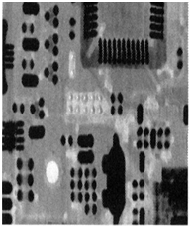
\includegraphics[width=0.3	\textwidth]{./Figures/cap3/eroded.png}}
	\caption{Erosión en imágenes en escala de grises (a) Imagen de entrada y (b) Imagen erosionada.}
	\label{fig:erosion}
\end{figure}


    \subsection{Apertura}
    La apertura tiene como función eliminar las protuberancias de la imagen, así como desconectar conjuntos y suprimir las componentes conexas más pequeñas que son cubiertas completamente por el elemento estructurante, matemáticamente la apertura se define como: 
    
       \begin{equation}
\label{eq:apertura}
 f(i,j) \circ{B} = (f(i,j)\ominus{B})\oplus{B}
\end{equation}
   
La expresión anterior no es más que la erosión de una imagen $f$ por un elemento estructurante $B$ seguido de una dilatación con el mismo elemento estructurante $B$. La FIGURA \ref{fig:apertura} muestra un ejemplo de la operación de apertura.

En la FIGURA \ref{fig:apertura1} se ve la imagen de un circuito y en la FIGURA \ref{fig:apertura2} se ve el resultado de aplicar la operación de apertura sobre dicha imagen, la cual  tiene un efecto suavizante sobre la imagen y suprime las partes pequeñas.

\begin{figure}[H]
	\centering
	 \subfigure[\label{fig:apertura1}]{	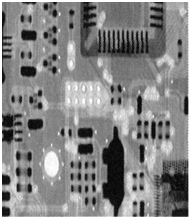
\includegraphics[width=0.3	\textwidth]{./Figures/cap3/gray1.png}}
	\subfigure[\label{fig:apertura2}]{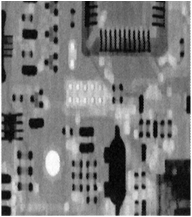
\includegraphics[width=0.3	\textwidth]{./Figures/cap3/opened.png}}
	\caption{Apertura en imágenes en escala de grises (a) Imagen de entrada y (b) Apertura de imagen.}
	\label{fig:apertura}
\end{figure}

    
    \subsection{Cierre}
    El cierre tiene como función  conectar  los  componentes cercanos  de  la  imagen  y  llenar  los huecos,   siempre   que   sean   más   pequeños   que   el   elemento   estructurante   empleado, matemáticamente el cierre se define como:
    
    \begin{equation}
\label{eq:cierre}
 f(i,j)\bullet{B}  = (f(i,j) \oplus{B})\ominus{B}
\end{equation}
    
   
    
    La expresión anterior representa una dilatación de la imagen  $A$ por un elemento estructurante $B$ seguida de una erosión con el mismo elemento estructurante  $B$. Las FIGURA \ref{fig:cierre}  muestra un ejemplo de la operación de cierre.
    
    En la FIGURA \ref{fig:cierre1} se ve la imagen de un circuito y en la FIGURA \ref{fig:cierre2} se ve el resultado de aplicar la operación de cierre sobre dicha imagen, la cual une los elementos pequeños de la imagen, y ha recubierto los agujeros y huecos pequeños.

\begin{figure}[H]
	\centering
	 \subfigure[\label{fig:cierre1}]{	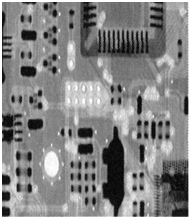
\includegraphics[width=0.3	\textwidth]{./Figures/cap3/gray1.png}}
	\subfigure[\label{fig:cierre2}]{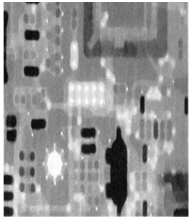
\includegraphics[width=0.3	\textwidth]{./Figures/cap3/closed.png}}
	\caption{Cierre en imágenes en escala de grises (a) Imagen de entrada y (b) Cierre de imagen.}
	\label{fig:cierre}
\end{figure}
    

\section{Transformada de Top-hat} 
La transformada de Top-hat es una operación que extrae pequeños elementos y detalles de las imágenes. La transformada de Top-hat $T_{w}$  \nomenclature[26]{$T_{w}$}{Función Transformada de Top-Hat.}
se utiliza para diversas tareas de visión por computadora, tales como la extracción de características, fondo de igualación, mejora de la imagen, y otros \cite{dougherty2003hands}.
La transformada de Top-hat es usada para objetos claros en fondos oscuros. La transformada de Top-hat de la imagen $f$ se define como la resta de la imagen $f$ con la apertura de $f$ con un elemento estructurante B, es decir:

\begin{equation}
\label{eq:tophatTrans}
T_w(f(i,j))=f(i,j) - (f(i,j) \circ B)
\end{equation}

  En la FIGURA \ref{fig:tophat1} se ve una imagen con pequeñas superficies claras y en la FIGURA \ref{fig:tophat2} se ve la imagen tras aplicar la operación de Top-hat, en la cual se puede ver estas superficies resaltadas con respecto al fondo de la imagen. 

\begin{figure}[H]
	\centering
	 \subfigure[\label{fig:tophat1}]{	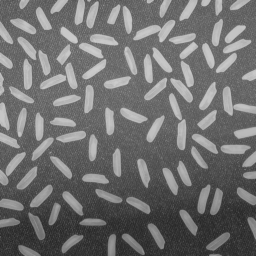
\includegraphics[width=0.3	\textwidth]{./Figures/cap3/rice.png}}
	\subfigure[\label{fig:tophat2}]{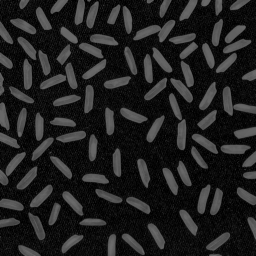
\includegraphics[width=0.3	\textwidth]{./Figures/cap3/rice_tophat.png}}
	\caption{Transformada de Top-Hat (a) Imagen de entrada y (b) Transformada de Top-Hat.}
	\label{fig:tophat}
\end{figure}

\section{Gradiente morfológico} 
El gradiente morfológico es útil en detección de bordes y aplicaciones de segmentación. De manera formal el gradiente morfológico de una imagen $f$ es la resta de la dilatación de la imagen $f$ por un elemento estructurante $B$ con la erosión de $f$ con un elemento estructurante $B$. La operación de gradiente morfológico se define como:
 %Gradiente morfológico es la diferencia entre la dilatación y la erosión de una imagen dada. Es útil en detección de bordes y aplicaciones de segmentación. 
 

\begin{equation}
\label{eq:gradienteMor}
Gr(f(i,j))=f(i,j)\oplus B-f(i,j)\ominus B
\end{equation}
\nomenclature[27]{$t$}{Nivel de intensidad de gris en el contexto de umbralización. }
\nomenclature[28]{$Gr$}{Función de Gradiente Morfológico.}%
En la FIGURA \ref{fig:gradiente1} se ve la imagen de un circuito y en la FIGURA \ref{fig:gradiente2} se ve la imagen con los bordes del circuito resaltados en un color más claro que se obtuvo tras aplicar la operación de gradiente morfológico sobre dicha imagen.

\begin{figure}[H]
	\centering
	 \subfigure[\label{fig:gradiente1}]{	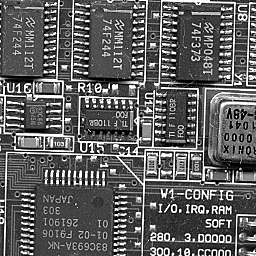
\includegraphics[width=0.3	\textwidth]{./Figures/cap3/gradiente.png}}
	\subfigure[\label{fig:gradiente2}]{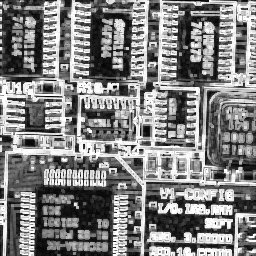
\includegraphics[width=0.3	\textwidth]{./Figures/cap3/gradiente2.png}}
	\caption{Gradiente morfológico (a) Imagen de entrada y (b) Gradiente morfológica.}
	\label{fig:gradiente}
\end{figure}


    
 %\section{Segmentación}
%La segmentación es el proceso de asignar una etiqueta a cada píxel de una imagen de tal manera que los píxeles con las mismas etiquetas comparten ciertas características visuales.
%El objetivo de la segmentación es simplificar y  la representación de una imagen en algo que es más significativo y más fácil de analizar \cite{shapirocomputer,barghout2003perceptual}. 

%La segmentación de imágenes permite dividir una imagen, para aislar segmentos, regiones u objetos individuales, que son homogéneos con respecto a algún rasgo; de tal forma que 
%se puedan extraer características o identificar y clasificar los objetos presentes en la imagen. 
%Estos datos pueden ser útiles para cuantificar regiones, tomar medidas sobre los objetos, discriminar  automáticamente los elementos presentes, definir bordes y  formas o diferenciar tonalidades \cite{molineroSegmentacion}. En la siguiente subsección se describe la segmentación por umbralización.
%Con base en ello, se han desarrollado  aplicaciones, por ejemplo, en imágenes de cultivos en agricultura \cite{molineroSegmentacion}.

\section{Segmentación por Umbralización}
En la literatura se reporta varios enfoques de segmentación \cite{abutaleb1988automatic}, de los cuales en este trabajo se utiliza la  segmentación por umbralización \emph{(thresholding)} que es un método que busca segmentar imágenes escalares creando una partición binaria de las intensidades de las imágenes \cite{coto2003metodos}.
Una umbralización trata de determinar un valor de intensidad, llamado umbral (\textit{threshold}), que separa la clases deseadas. La segmentación se logra agrupando todos los píxeles con mayor intensidad al umbral en una clase, y todos los otros píxeles en otra clase. Es útil cuando hay una clara diferencia entre los objetos a extraer respecto del fondo de la escena \cite{al2010image}.

Las técnicas de umbralización se pueden clasificar en dos clases:  global y local (adaptativa). En el umbral global, un solo valor de umbral es utilizado para toda la imagen. En cambio para los el umbrales locales, un valor umbral se asigna a cada píxel de manera a determinar si pertenece al primer plano o al fondo usando la información local alrededor del píxel. Debido a la simplicidad de la umbralización
global, esta ha sido una técnica popular en muchos años \cite{kittler1986minimum,huang1995image}.

En la FIGURA \ref{fig:segxumbra1} se ve una imagen en escala de grises con pequeñas superficies grises en forma de elipse y en la FIGURA \ref{fig:segxumbra2} se puede ver una imagen binaria donde el fondo de la imagen se distingue en negro y las pequeñas superficies en forma de elipse en blanco, esta imagen es resultado de umbralizar dicha imagen.

\begin{figure}[H]
	\centering
	 \subfigure[\label{fig:segxumbra1}]{	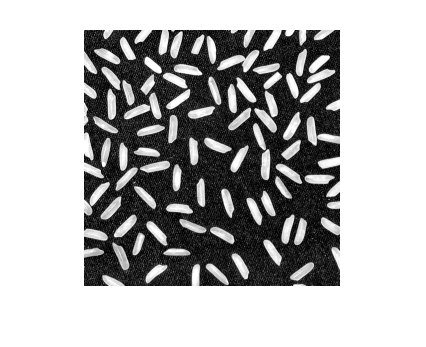
\includegraphics[width=0.4	\textwidth]{./Figures/cap3/SegThresh_01.png}}
	\subfigure[\label{fig:segxumbra2}]{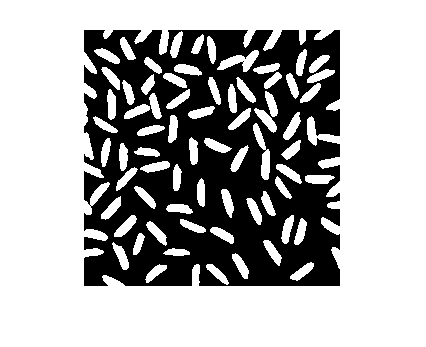
\includegraphics[width=0.4	\textwidth]{./Figures/cap3/SegThresh_02.png}}
	\caption{Segmentación por umbralización (a) Imagen de entrada y (b) Imagen segmentada.}
	\label{fig:segxumbra}
\end{figure}


  % \section{Umbralización} 
  % Los métodos del valor umbral separan los objetos de una imagen que nos interesen del resto. Con la ayuda de los métodos de valor umbral en las situaciones más sencillas se puede decidir qué píxeles conforman los objetos que buscamos y qué píxeles son sólo el entorno de estos objetos \cite{gonzales2002digital}.  
   
   %Normalmente los métodos del valor umbral "binarizan" la imagen de partida, es decir se construyen dos segmentos: el fondo de la imagen y los objetos. La asignación de un pixel a uno de los dos segmentos (0 y 1) se consigue comparando su nivel de gris g con un cierto valor umbral preestablecido t (en inglés threshold).\cite{gonzales2002digital}. La imagen final es muy sencilla de calcular ya que para cada pixel sólo hay que realizar una comparación numérica. La regla de cálculo correspondiente $T_g$ es:
Los métodos de umbralización usados en este trabajo son el Otsu \cite{otsu1975threshold} y entropía máxima \cite{cattaneo2011metodos}, los cuales se explican en las siguientes secciones.
\subsection{Otsu}
El método de Otsu, llamado así en honor a su creador Nobuyuki Otsu \cite{otsu1975threshold}, calcula el valor umbral de forma que la dispersión (distancia entre los valores respecto a un valor medio) dentro de cada segmento sea lo más pequeña posible, pero al mismo tiempo la dispersión sea lo más alta posible entre segmentos diferentes. Para ello se calcula el cociente entre ambas varianzas y se busca un valor umbral de intensidad para el que este cociente sea máximo \cite{gonzalez2013tecnicas}. 
Como punto de partida se toma dos segmentos de intensidades $S_0(t)$  y $S_1(t)$, que serán definidos a partir del valor umbral $t$. Dónde $t$ es la variable que se busca, y los dos segmentos son el resultado deseado en la segmentación. 

Sea $p(k)$ la probabilidad de ocurrencia del valor de gris, $0 \leq k \leq  F_{max}$. Entonces la probabilidad de ocurrencia de los píxeles en los dos segmentos es \cite{gonzalez1992digital}:
\nomenclature[29]{$S_{0}(t)$}{Conjunto de valores de intensidades menores o iguales a $t$ en una imagen $f$.}%
\nomenclature[30]{$S_{1}(t)$}{Conjunto de valores de intensidades mayores a $t$ en una imagen $f$.}%


\begin{equation}S_{0}:p_{0}(t) = \sum_{k=0}^t p(k)\end{equation} y \begin{equation}S_{1}:p_{1}(t)= \sum_{k=t+1}^{F_{max}} p(k) = 1-p_{0}(t)\end{equation}


siendo $F_{max}=L-1$ y valor de gris máximo. Cabe mencionar que si se toman los dos segmentos la suma de las probabilidades dará evidentemente 1.

Si $\overline{k}$  es la media aritmética de los valores de gris en toda la imagen, y $\overline{k_0}$
 y $\overline{k_1}$  los valores medios dentro de cada segmento, entonces se pueden calcular las varianzas dentro de cada segmento como:
\nomenclature[31]{$\overline{k}$}{Media aritmética de los valores de gris en la imagen.}%
\nomenclature[32]{$\overline{k_0}$}{Media aritmética de los valores de gris en $S_0$.}%
\nomenclature[33]{$\overline{k_1}$}{Media aritmética de los valores de gris en $S_1$.}%

\begin{equation}\sigma_0^2(t) = \sum_{k = 0}^t(k - \overline{k_{0}})^2p(k)\end{equation} y 

\begin{equation}
\sigma_1^2(t) = \sum_{k = t + 1}^{F_{max}}(k - \overline{k_{1}})^2p(k)\end{equation}
\nomenclature[34]{$\sigma_0^2$}{Varianza de la intensidades en $S_0$.}%
\nomenclature[35]{$\sigma_1^2$}{Varianza de la intensidades en $S_1$.}%
El objetivo final es mantener la varianza dentro de cada segmento $\sigma_{in}^2(t)$ lo más pequeña posible y conseguir que la varianza entre los dos segmentos $\sigma_{zw}^2(t)$ sea lo más grande posible. Así define el parámetro $Q(t)$ como la relación entre varianzas:
\begin{equation}Q(t)=\frac{\sigma_{zw}^2(t)}{\sigma_{in}^2(t)}\end{equation}
\nomenclature[36]{$Q(t)$}{Relación entre varianzas.}%
La varianza entre los segmentos es:

\begin{equation}\sigma_{zw}^2(t) = p_0(t)\cdot(\overline{k_0} - \overline{k})^2 + p_1(t)\cdot(\overline{k_1} - \overline{k})^2\end{equation}

La varianza dentro de los segmentos se obtiene de la suma de ambas: 

\begin{equation}
\sigma_{in}^2(t) = p_0(t)\cdot\sigma_0^2(t) + p_1(t)\cdot\sigma_1^2(t)\end{equation}

\nomenclature[37]{$\sigma_{in}^2(t)$}{Varianza entre $S_0$ y $S_1$.}%
\nomenclature[38]{$\sigma_{zw}^2(t)$}{Varianza dentro de los segmentos $S_0$ y $S_1$.}%
El valor umbral $t$ se elige de manera que el cociente $Q(t)$ sea máximo. $Q(t)$ es por lo tanto la medida buscada. De esta forma se elige un valor umbral que optimiza los dos segmentos en términos de varianza \cite{gonzalez2013tecnicas}. En la FIGURA \ref{fig:otsu1} se ve la imagen  de una mujer en escala de grises y en la FIGURA \ref{fig:otsu2} se muestra una imagen binaria en donde se puede notar que solo las zonas más oscuras de la imagen se pusieron negras y las zonas más claras cambiaron por blanco, esta imagen es  resultado de aplicar la umbralización por el método de Otsu. Este algoritmo de umbralización se usa en la detección y segmentación de borde circular porque diferencia claramente el fondo que suele ser una zona más oscura con respecto a la retina.
    \begin{figure}[H]
	\centering
	 \subfigure[\label{fig:otsu1}]{	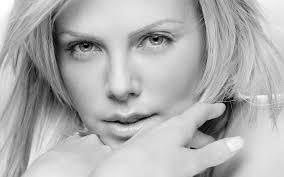
\includegraphics[width=0.3	\textwidth]{./Figures/cap2/umbral.jpg}}
	\subfigure[\label{fig:otsu2}]{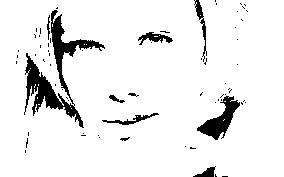
\includegraphics[width=0.3	\textwidth]{./Figures/cap2/umbralo.jpg}}
	\caption{Método de Otsu (a) Imagen en escala de grises y (b) Imagen umbralizada.}
	\label{fig:otsu}
\end{figure}
\subsection{Entropía Maxima}

Los métodos de binarización basados en la entropía usan la entropía de los niveles de gris en una imagen. La máxima entropía es interpretada como la máxima información 
transferida y es el umbral óptimo \cite{cattaneo2011metodos}.

$H(k)$ denota el valor de un histograma normalizado. Típicamente $k$ toma valores del $F_0$ a $F_{max}$. Se asume que $H(k)$  esta normalizado

\begin{equation}
\label{eq:histograma}
\sum_{k=0}^{F_{max}}H(k)=1
\end{equation}

La entropía de los píxeles negros para el nivel de intensidad $t$ se define como:


\begin{equation}
\label{eq:entropiaBlancos}
E_1(t)=-\sum_{k=0}^{t} \frac{H(k)}{\sum_{l=0}^{t}H(l)} \log \frac{H(k)}{\sum_{l=0}^{t}H(l)}
\end{equation}
\nomenclature[39]{$E_1(t)$}{Entropía de los píxeles de intensidades menores o igual a $t$.}%

La entropía de los píxeles blancos para el nivel de intensidad $t$ se define como:


\begin{equation}
\label{eq:entropiaNegro}
E_2(t)=-\sum_{k=t+1}^{F_{max}} \frac{H(k)}{\sum_{l=t+1}^{F_{max}}H(l)}\log
\frac{H(k)}{\sum_{l=t+1}^{F_{max}}}H(l)
\end{equation}
\nomenclature[40]{$E_2(t)$}{Entropía de los píxeles de intensidades mayores a $t$.}%

\nomenclature[41]{$T$}{Valor de intensidad óptimo en la umbralización de entropía máxima.}%
El umbral óptimo $T$ es seleccionado encontrando el argumento $t$  que maximice la ecuación (\ref{eq:umbralMaxEntrop})

\begin{equation}
\label{eq:umbralMaxEntrop}
T= \underset{t\in [F_0,F_{max}]}{\operatorname{arg\,max}} \;\{E_1(t)+E_2(t)\}
\end{equation}
La FIGURA \ref{fig:maxentropia1} se ve la imagen en escala de escala de grises de una mujer y en la FIGURA \ref{fig:maxentropia2} se ve una imagen binaria en donde se ve que las zonas oscuras y ciertas zonas claras del cabello se pusieron en negro en cambio en el método de Otsu solo las zonas más oscuras se pusieron en negro. Este algoritmo de umbralización se utiliza en la segmentación de patologías y estructuras anatómicas del ojo porque permite detectar otras zonas a parte del fondo.
  \begin{figure}[H]
	\centering
	 \subfigure[\label{fig:maxentropia1}]{	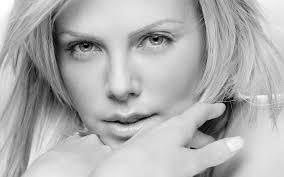
\includegraphics[width=0.3	\textwidth]{./Figures/cap2/umbral.jpg}}
	\subfigure[\label{fig:maxentropia2}]{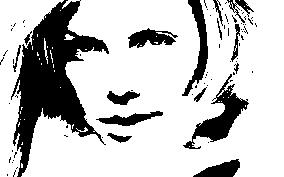
\includegraphics[width=0.3	\textwidth]{./Figures/cap2/umbralm.jpg}}
	\caption{Entropía Maxima (a) Imagen en escala de grises y (b) Imagen umbralizada.}
	\label{fig:maxentropia}
\end{figure}


\section{Extracción de Características}
Una vez realizado el proceso de segmentación, el  siguiente  paso  consiste en obtener que características que definan los objetos segmentados, por ejemplo: forma, textura, color y orientación. Los algoritmos 
usados en esta etapa dependen de la aplicación requerida \cite{nayak2008automated,qiu2005image,cui2008edge}.

Generalmente el proceso de extracción de características agrega las características cuantitativas en un vector de características \cite{wernick2010machine}.


%En reconocimiento de patrones y aprendizaje supervisado, un vector característica es un vector n-dimensional de características numéricas que representan algún objeto. Muchos algoritmos de aprendizaje de máquina requieren una representación numérica de los objetos, ya que tales representaciones facilitan el procesamiento y análisis estadístico \cite{piramuthu2009iterative}.


%Al representar las imágenes, los valores de características podrían corresponder a los píxeles de una imagen, al representar los textos tal vez para frecuencias de ocurrencias. Los vectores de características son equivalentes a los vectores de variables explicativas utilizadas en procedimientos estadísticos como la regresión lineal.

En nuestro caso las imágenes  obtenidas al final las segmentaciones son imágenes binarias que contienen los objetos de interés. La característica utilizada es la sumatoria de las áreas de los objetos segmentados que son los microaneurismas, exudados duros y vasos sanguíneos.
%o componentes conectados. 
%Entre las características de objetos binarios incluyen: área, área central,  el perímetro, el número de Euler, las proyecciones y la proporción de la delgadez.




%Más adelante se dará más detalles sobre la extracción del área del objeto de interés.
 

%\section{Clasificador SVM}
%Las máquinas de soporte vectorial o máquinas de vectores de soporte (Support Vector Machines, SVMs) tienen su fundamento en la teoría estadística del aprendizaje desarrollada por el grupo de Vladimir Vapnik \cite{cortes1995support}. Dado $n$ muestras o vectores de entrenamiento representadas mediante pares $(x_{i},y_{i})$, donde $y_{i}$ es la etiqueta de clase $(y_{i} \in \{1,-1\})$ y $x_{i}$ el vector de atributos $(i = 1,...,n)$; en el caso ideal (2 clases completamente separables) existe un número infínito de planos (o hiperplanos) que pueden separar las dos clases. El objetivo de las SVMs es encontrar el hiperplano que separe las dos clases y que simultáneamente esté lo más lejano posible de los patrones de entrenamiento más cercanos (FIGURA \ref{fig:svm}) \cite{cortes1995support,burges1998tutorial}.
 % \begin{figure}[H]
%	\centering
%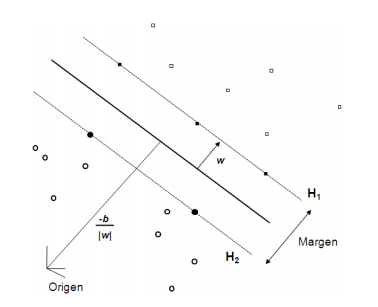
\includegraphics[width=0.6	\textwidth]{./Figures/cap3/svm.png}

%	\caption{Margen entre el hiperplano separador y los vectores soporte}
%	\label{fig:svm}
%\end{figure}

%Está demostrado, en el caso ideal, que la probabilidad de cometer un error ante una muestra desconocida (test) está acotada por la relación entre valor esperado de vectores soporte y el número de vectores de entrenamiento. Además, la función de clasificación puede ser construida a partir de un número bajo de vectores soporte, respecto al número de vectores de entrenamiento, la capacidad de generalización del clasificador será alta, aún en un espacio de separación de dimensiones infinitas \cite{cortes1995support}.

%Formalmente, la función de clasificación (hiperplano óptimo) son los puntos que satisfacen:
%\begin{equation}
%\label{eq:svm2.2}
%w.x_{i} \pm b =0
%\end{equation}
%\textbf{w} es un vector normal al hiperplano, $\left | b \right |/\left \| \textbf{w} \right \|$ es la distancia perpendicular del
%hiperplano al origen y $\left \| \textbf{w} \right \|$ es la norma euclídea de \textbf{w} \cite{burges1998tutorial}. Siendo $d_{+}(d_{-})$ la distancia del hiperplano al ejemplo más cercano, se define como margen a la suma $d_{+}+d_{-}$ (FIGURA \ref{fig:svm}). Como resultado, los datos de entrenamiento satisfacen:
%\begin{equation}
%\label{eq:svm2.3}
%x_{i}.w\pm b \geqslant +1  \textup{ para }  y_{i}= 1 (C_{1})
%\end{equation}

%\begin{equation}
%\label{eq:svm2.4}
%x_{i}.w \pm b \leqslant   -1  \textup{ para }  y_{i}= -1 (C_{1})
%\end{equation}
%Si se elige una escala adecuada para $\textbf{w}$ y $b$, los puntos que satisfacen la igualdad de la ecuación \ref{eq:svm2.3} estarán ubicados sobre el hiperplano $H_{1}:x_{i}.\textbf{w} + b =1$ con vector normal \textbf{w} y distancia al origen $\left |1- b \right |/\left \| \textbf{w} \right \|$ (hiperplano soporte). De la misma manera, los puntos que satisfacen la igualdad de ecuación \ref{eq:svm2.4} están ubicados en el hiperplano $H_{2}:x_{i}.\textbf{w} + b =-1$ , con vector normal \textbf{w} y distancia perpendicular al origen $\left |-1- b \right |/\left \| \textbf{w} \right \|$. En consecuencia, $(d_{+}=d_{-}=\left\| \textbf{w} \right \|$ y el margen es igual a $2/\left\| \textbf{w} \right \|)$. Finalmente, para encontrar el par de hiperplanos $H_{1}$ y $H_{2}$ con mayor margen se busca minimizar:
%\begin{equation}
%\label{eq:svm2.5}
%\frac{1}{2}\left \| w \right \|^{2}
%\end{equation}
%Sujeto a las restricciones \ref{eq:svm2.3} y \ref{eq:svm2.4}.

%El anterior es un problema de optimización cuadrático cuya solución explícita es difícil de obtener \cite{burges1998tutorial}. Utilizando Multiplicadores de Lagrange la solución es maximizar:

%\begin{equation}
%\label{eq:svm2.6}
%(\alpha)=\sum_{i=1}^{n} \alpha_{1} - \frac{1}{2}\sum_{i=1}^{n}\sum_{j=1}^{n}\alpha_{i}\alpha_{j}y_{i}y_{j} \mathbf{x}_{i}.\mathbf{x}_{j}
%\end{equation}

%sujeto a 
%\begin{equation}
%\label{eq:svm2.7}
%\sum_{i=1}^{n}\alpha_{i}y_{i}
%\end{equation}
%y
%\begin{equation}
%\label{eq:svm2.8}
%0 \leqslant  \alpha_{i}
%\end{equation}

%Los elementos $\alpha_{i}$ son los multiplicadores de Lagrange, los vectores soporte corresponden a aquellos puntos donde $\alpha_{i} > 0$ mientras que $\alpha_{i}= 0$ indica los puntos de entrenamiento que están ubicados fuera del espacio limitado por $H_{1}$ y $H_{2}$.
%En situaciones reales, donde algunos de los datos de $C_{1}$ y $C_{2}$ se superponen, se deben relajar ciertas restricciones para poder hallar una función de clasificación robusta. Dicho de otra manera, ante la presencia de datos atípicos (\emph{outliers} ), es imposible encontrar una hiperplano que separe todos los puntos de entrenamiento. En
%este caso se prefiere que la mayoría de los puntos esté correctamente clasificados y el resto (\emph{outliers}) estará ubicado en el lado incorrecto del hiperplano separador. Consecuentemente, el problema de optimización se modela no sólo para maximizar el margen entre los planos soporte sino también para minimizar los errores de clasificación. Con este fin se introducen variables de "holgura" (\emph{slack variables}) no negativas ($\zeta_{i}$) de tal manera que \cite{burges1998tutorial}:

%\begin{equation}
%\label{eq:svm2.9}
%x_{i}.w\pm b \geqslant +1  - \zeta_{i} \textup{ para }  y_{i}= +1
%\end{equation}
%y
%\begin{equation}
%\label{eq:svm2.10}
%x_{i}.w \pm b \leqslant   -1  - \zeta_{i}  \textup{ para }  y_{i}= -1
%\end{equation}
%Para obtener el hiperplano óptimo la solución es:
%\begin{equation}
%\label{eq:svm2.11}
%\texttt{minimizar}\frac{1}{2}\left \| w \right \|^{2} +  C\sum_{i=1}^{n}\zeta_{i}
%\end{equation}
%o máximizar la expresión \ref{eq:svm2.6} sujeto a
%\begin{equation}
%\label{eq:svm2.12}
%\sum_{i=1}^{n}\alpha_{i}y_{i}=0
%\end{equation}
%y
%\begin{equation}
%\label{eq:svm2.13}
%0 \leqslant \alpha_{i}y_{i} \leqslant  C
%\end{equation}

%El parámetro $C$ (parámetro de costo) involucra una solución de compromiso entre el margen de los dos planos soporte y el error de clasificación y determina cuan severamente se penalizan los errores de clasificación durante el entrenamiento \cite{cortes1995support,burges1998tutorial}. Finalmente, como en el caso ideal, la solución del hiplerplano óptimo será:
%\begin{equation}
%\label{eq:svm2.14}
%w=\sum_{i=1}^{n_{s}}\alpha_{i}y_{i}\mathbf{x_{i}}
%\end{equation}
%donde $n_{s}$ es el número de vectores soporte.
%Cuando las muestras de entrenamiento no son linealmente separables, en vez de generar una curva no lineal para clasificar los datos, el algoritmo utiliza una función $\Phi(x_{i})$ para mapear los valores de entrada a un espacio con mayor número de dimensiones (espacio de caracteríticas o \emph{features}) y con el objeto de poder computar una separación lineal confiable (FIGURA \ref{fig:svmnlin}). En este caso la ecuación del hiperplano óptimo puede ser enunciada como:
%  \begin{figure}[H]
%	\centering
%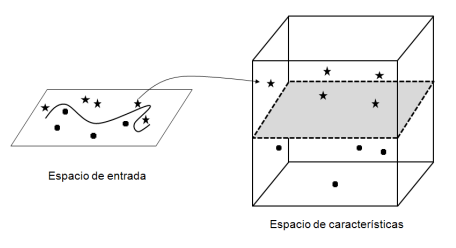
\includegraphics[width=0.6	%\textwidth]{./Figures/cap3/mapeonolinealsvm.png}

%	\caption{Mapeo no lineal del espacio de entrada al espacio de características}
%	\label{fig:svmnlin}
%\end{figure}

%\begin{equation}
%\label{eq:svm2.15}
%f(\mathbf{x})=\sum_{i=1}^{n_{s}}\alpha_{i}y_{i} \Phi(\mathbf{x_{i}}).\Phi(\mathbf{x}) +b
%\end{equation}
%Dado que no siempre es posible una solución directa se emplea una función kernel, en consecuencia la ecuación del hiperplano se puede expresar como:
%\begin{equation}
%f(\mathbf{x})=\sum_{i=1}^{n_{s}}\alpha_{i}y_{i}K(\mathbf{x_{i}},\mathbf{x}) + b
%\end{equation}
%,
%\begin{equation}
%\label{eq:svm2.17}
%K(\mathbf{x_{i},x_{j}})=< \phi (\mathbf{x_{i}}),\phi (\mathbf{x_{j}})> 
%\end{equation}

%Los kernels más utilizados son: polinomial, sigmoideo y función de base radial o RBF (radial basis function).

%El kernel lineal se puede expresar como:
%\begin{equation}
%K(\mathbf{x_{i},x_{j}})=(\mathbf{x_{i}-x{j}})
%\end{equation}
%mientras que en el kernel de función de base radial,
%\begin{equation}
%K(\mathbf{x_{i},x_{j}})=e^{-\gamma{(\mathbf{x_{i}-x{j}})}^{2}}
%\end{equation}

%Si bien existen extensiones del concepto clásico de SVMs que %permiten realizar clasificación multiclase\cite{lee2004multicategory} en este trabajo de tesis sólo se utilizan las versiones binarias \cite{platt1998machines,keerthi2001improvements}.


\section{Clasificador SVM}
Las máquinas de soporte vectorial o máquinas de vectores de soporte (SVM por su nombre en inglés \textit{Support Vector Machines}) tienen su fundamento en la teoría estadística del aprendizaje desarrollada por el grupo de Vladimir Vapnik \cite{cortes1995support,boser1992training}. Es un método de aprendizaje automático que intenta tomar datos de entrada y clasificarlos en una de dos categorías.
 
Para que una máquina de vectores de soporte sea efectiva, es necesario un conjunto de datos de entrenamiento (datos de entrada y salida)  para construir el modelo que pueda clasificar nuevos datos, dibujándolos en un espacio multidimensional, y después usando regresión para encontrar un hiperplano (una superficie en un espacio dimensional $n_{D}$ que separa el espacio en dos semiespacios) que separa de la mejor manera las dos clases de entrada, con el cual es capaz de clasificar las nuevas entradas en una de las dos categorías.

%En la FIGURA \ref{fig:svmSeparacionHiperplano}  se observa el funcionamiento del clasificador, los círculos rojos y las cruces azules se usan para denotar los dos tipos de entrada, con una línea negra indicando el hiperplano separador. Cada uno de los datos individuales tienen un valor de entrada única 1 (representado por su posición en el eje x) y un valor de entrada única 2 (representado por su posición en el eje y).
 % \begin{figure}[H]
%	\centering
%	 \subfigure[]{	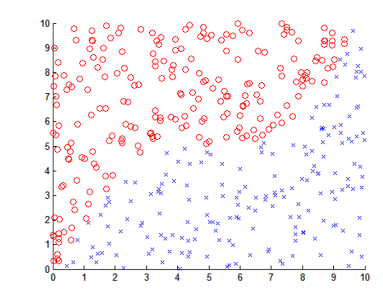
\includegraphics[width=0.45	\textwidth]{./Figures/cap3/separacionHiperplano1.png}}
%	\subfigure[]{\includegraphics[width=0.45	\textwidth]{./Figures/cap3/separacionHiperplano2.png}}
%	\caption{Ejemplo del SVM (a) Tipos de entrada y (b) Hiperplano separador}
%	\label{fig:svmSeparacionHiperplano}
%\end{figure}


Si bien existen extensiones del concepto clásico de SVM que permiten realizar clasificación multiclase \cite{lee2004multicategory,platt1998machines,keerthi2001improvements} en este trabajo sólo se utiliza la versión binaria. A continuación se describe el funcionamiento del clasificador SVM de kernel lineal que se utiliza en este trabajo.


El clasificador SVM  recibe un conjunto de entrenamiento  $D$, compuesto por $v$ puntos de la forma
\nomenclature[42]{$D$}{Conjunto de entrenamiento del clasificador SVM.}
\nomenclature[43]{$x_i$}{Vector de p-dimensional a clasificarse.}
\nomenclature[44]{$y_i$}{Grupo al cual pertenece $x_i$.}
%\nomenclature[]{$w$}{Normal al hiperplano.}
\begin{equation} \label{eq:svm1}
D = \{ (x_i, y_i)\}_{i=1}^v
\end{equation}

donde $x_{i}$ es un vector p-dimensional, e $y_i$ denota el grupo al cual pertenece $x_{i}$. Como se trata de un clasificador binario $y_i$ solo puede tener dos grupos posibles:

\begin{equation} \label{eq:svm2}
y_i \in \{1,-1\}
\end{equation}

\nomenclature[45]{$w$}{Normal al hiperplano.}
\nomenclature[46]{$x$}{Conjunto de puntos de entrenamiento.}
Se busca dos hiperplanos de tal manera que los datos esten separados en sus respectivos grupos y no exista punto entre ellos. La región entre estos hiperplanos es conocida como margen. Estos hiperplanos son descritos como sigue:

\begin{equation} \label{eq:svm4}
w\cdot x -b =1
\end{equation}
y 
\begin{equation} \label{eq:svm41}
w\cdot x -b =-1
\end{equation}

donde $w$ denota la normal al hiperplano, $x=\{x_1,...x_n\}$ es el conjunto de puntos de entrenamiento y el $\frac{b}{\left \| w \right \|}$ determina el desplazamiento del hiperplano del origen hacia el vector normal.

\nomenclature[47]{$\frac{b}{\left \| w \right \|}$}{Desplazamiento del hiperplano del origen hacia el vector normal.}

Usando geometría se busca que la distancia entre los dos hiperplanos sea $\frac{2}{\left \| w \right \|}$ (Ver FIGURA \ref{fig:svm2}). 


\begin{figure}[H]
	\centering
		\includegraphics[width=0.4	\textwidth]{./Figures/cap3/svm2.png}
	\caption{Distancia entre hiperplanos.}
	\label{fig:svm2}
\end{figure}


Para evitar que los puntos de los datos de entrenamiento se encuentren dentro del margen se agrega las siguientes restricciones:

\begin{equation} \label{eq:svm5}
w\cdot x_i-b\geq 1 \rightarrow  \text{para todo } x_i \text{ del primer grupo }
\end{equation}

y
\begin{equation} \label{eq:svm55}
w\cdot x_i-b\leq -1 \rightarrow  \text{para todo } x_i \text{ del segundo grupo }
\end{equation}
Esto puede ser reformulado como sigue:

\begin{equation} \label{eq:svm12}
y_i(w\cdot x_i-b)\geq 1, \forall i \in \{1,..,n\}
\end{equation}

Se busca minimizar $\left \| w \right \|$ sujeto a la restricción (\ref{eq:svm12}) de tal manera a obtener la $w$ óptima.



Una vez obtenida la w óptima, el clasificador SVM con kernel lineal (Ver FIGURA \ref{fig:svm1}) tendrá la forma:

\begin{equation} \label{eq:svm3}
CL(x_c)=w\cdot x_c +b
\end{equation}

\nomenclature[49]{$CL$}{Función del clasificador \textit{SVM}.}

\nomenclature[48]{$x_c$}{Punto a clasificar.}
En donde $x_c$ representa el punto que se quiere clasificar y los valores de $CL(x_c)$ determinan el grupo al cual va pertenecer el punto $x_c$.

\begin{equation} \label{eq:svm6}
\begin{cases}
 & CL(x)\geq 0 \rightarrow  y_i=+1\\ 
 & CL(x)<  0 \rightarrow  y_i=-1
\end{cases}
\end{equation}

\begin{figure}[H]
	\centering
		\includegraphics[width=0.5	\textwidth]{./Figures/cap3/svmv.png}
	\caption{Clasificador SVM con kernel lineal.}
	\label{fig:svm1}
\end{figure}

\section{Resumen}


En este capítulo se explica los conceptos de visión por computadora utilizados en la metodología propuesta. La representación de imagen a utilizarse es definida, además se muestra el espacio de color en el cual se estará trabajando. Se define conceptos de vecindad de un píxel, conectividad y componentes conectados. 
Con respecto al pre-procesamiento de imágenes se comenta los conceptos de filtros, ecualización del histograma, ajuste de valores de intensidad y transformada de hough. En relación a la morfología matemática primeramente se define un elemento estructurante, luego se formula las operaciones de dilatación, erosión, clausura y cierre tanto para imágenes binarias y en escala de grises. La segmentación por umbralización se detalla y se hace una breve reseña sobre los algoritmos de umbralización: Otsu y entropía máxima. Finalmente, se explica la extracción de características y el funcionamiento del clasificador binario SVM de kernel lineal.
En el siguiente capítulo se presenta la metodología propuesta y se explica de manera detallada sus módulos.